\documentclass{article}

\usepackage{amsmath,amsfonts, amssymb,wasysym, latexsym, hyperref, mathdots, enumerate, pstricks,setspace,epsfig,amsthm}
\usepackage{tikz}
\usetikzlibrary{calc}
\usetikzlibrary{shapes}
\usetikzlibrary{arrows}
\usetikzlibrary{backgrounds}

\usepackage{todonotes}

\usepackage{graphicx,times}
\usepackage[toc,page]{appendix}
\usepackage{fullpage}
\usepackage[parfill]{parskip}
\usepackage{subfig}
\usepackage{caption}
\usepackage[figuresleft]{rotating}
\usepackage{float}
\usepackage{multibib}
\usepackage{makecell}
\usepackage{booktabs}
\usepackage{longtable}
\usepackage{ragged2e}
\usepackage{setspace}
\usepackage{color}

% New commands------------------------
\newcommand{\NH}{\text{NH}}
\newcommand{\RG}{\text{RG}}
\newcommand{\todoVK}[1]{\todo[color=blue!20]{#1}}


\title{Measuring the Price of Anarchy in Critical Care Unit Interactions}
\author{Vincent Knight*
    \and
        Izabela Komenda
    \and
        Jeff Griffiths}

\begin{document}
\maketitle

\begin{abstract}
Hospital throughput is often studied and optimised in isolation, ignoring the interactions between hospitals.
In this paper Critical Care Unit (CCU) interaction is placed within a game theoretic framework.
The methodology involves the use of a normal form game underpinned by a two dimensional continuous Markov chain.
A theorem is given that proves that a Nash Equilibrium exists in pure strategies for the games considered.

The effect of target policies is investigated justifying the use of these to align the interests of individual hospitals and social welfare.
In particular, we identify the lowest value of a utilisation target that aligns these.
\end{abstract}

\section{Introduction}

A Critical Care Unit (CCU), also sometimes referred to as an Intensive Therapy Unit or Intensive Therapy Department, is a special ward that is found in most acute hospitals.
It provides intensive care (treatment and monitoring) for people who are critically ill or are in an unstable condition.
CCUs face major challenges.
The first challenge that CCUs have to deal with is shortage of beds.  On average, 8\% of patients are refused admission to a CCU because the Unit is full \cite{Report}. The CCU occupancy rates for some hospitals are reportedly very high \cite{Mitchell1995,Smith1995} and a shortage of beds has been identified throughout the UK.

Patients in CCUs need constant medical support to keep their body functioning.
Moreover, CCU beds are very expensive and a limited resource; therefore efficient CCU bed management is crucial.
Many previous researchers have developed queueing models to help manage bed capacities in hospitals \cite{Cooper1974,Dumas1984,Gallivan2011,Gorunescu2002a,Griffiths2012,Harper2002a}.
Also, a vast amount of literature has been devoted to simulation of CCUs;  \cite{Cahill1999a,Costa2003,Griffiths2004a,Kim1999,Litvak2008,Shahani2008}.

This paper describes part of a project undertaken with managers from the Aneurin Bevan University Health Board (ABUHB), which is an NHS Wales organization in South Wales, that serves 21\% of the total population of Wales \cite{Board}.
Critical care is delivered on two sites, at the Nevill Hall hospital in Abergavenny and at the Royal Gwent hospital in Newport.
For the remainder of this paper, the Nevill Hall hospital will be referred to as NH and the Royal Gwent hospital as RG.

The main proposition of the work requested by the ABUHB was to develop a mathematical model of bed occupancies at the CCUs at RG and NH.
After an initial analysis of the data, behavioural aspects became apparent; for example, delaying patients discharge if there was no pressure on CCU beds, or admitting fewer patients if bed occupancy levels were high.
As a result of this, a state-dependent queueing model has been developed, which includes the dependency of admission rate on actual occupancy \cite{Komenda2013}.
This state dependent model was applied to both NH and RG separately.
It is however obvious that the actions of one CCU impact on the other CCU, as diversion of patients from one CCU to the other sometimes occurs.
A pictorial representation of the situation is given in Figure \ref{diagramofdiversion}.

\begin{figure}[!htbp]
\begin{center}
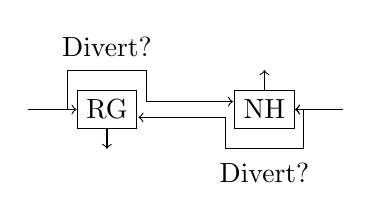
\begin{tikzpicture}
\node (A) at (0,0) [draw] {RG};
\node (B) at (2,0) [draw] {NH};
\draw [->] (-1,0) -- (A);
\draw [->] (3,0) -- (B);
\draw [->] (-1,0) -- ($(A)+(-.5,0)$) -- ($(A)+(-.5,.5)$) -- ($(A)+(.5,.5)$) -- ($(A)+(.5,.1)$) -- ($(B)+(-.4,.1)$);
\draw [->] (3,0) -- ($(B)+(.5,0)$) -- ($(B)+(.5,-.5)$) -- ($(B)+(-.5,-.5)$) -- ($(B)+(-.5,-.1)$) -- ($(A)+(.4,-.1)$);
\draw [->] (3,0) -- (B);
\node at ($(A) + (0,.8)$) {Divert?};
\node at ($(B) + (0,-.8)$) {Divert?};
\draw [->] (A) -- ($(A)+(0,-.5)$);
\draw [->] (B) -- ($(B)+(0,.5)$);
\end{tikzpicture}
\caption{Diagrammatic representation of CCU interaction through patient diversion.}\label{diagramofdiversion}
\end{center}
\end{figure}

Game theory is the mathematical study of interactive decision making between rational decision makers \cite{Maschler2013}.
A game is a description of strategic interactions that includes the constraints on the actions that the players can take and on the players' interests.

Most research where game theory is applied in healthcare has mainly concentrated on Emergency Departments (EDs) and how to deal with diversions of patients and ambulances.
In \cite{Hagtvedt2009} cooperative strategies for hospitals are considered, in order to reduce occurrences when ambulances are turned away due to the ED being full.
In \cite{Deo2011} a queueing network model of two EDs is proposed to study the network effect of ambulance diversion.
Each ED aims to minimise the expected waiting time of its patients (walk-ins and ambulances) and chooses its diversion threshold based on the number of patients at its location. Decentralised decision making in the network is modelled as a non-cooperative game.

Some other work that has not concentrated on EDs, but has been applied to healthcare includes: \cite{Knight2013}, where results concerning the congestion related implications of decisions made by patients when choosing between healthcare facilities were presented. In \cite{Howard2002} a model of the accept/reject decision for transplant organs is developed.

In the wider intersection of game theory and queueing theory (where this work lies) papers that consider price and/or capacity include: \cite{Allon2007, Cachon2002,  Cachon2007, Kalai1992, Levhari1978}. In these models, the choice of price/or capacity determines the arrival rate for each firm; this is similar to the approach taken in this paper.

The work presented in this paper contributes to the growing body of literature by applying state dependent queueing models in a game theoretical context to CCU interaction.
In particular this consideration allows for the investigation of targets imposed by central control \cite{Bevan2006}.
The findings of this work justify and identify a choice of targets that align the interests of the individual hospitals with social welfare.

The data used for the work presented in this paper was provided by the Intensive Care National Audit and Research Centre (ICNARC) and refers to patients admitted to CCUs in NH and RG, and covers a period of three years, from the 1$^{\text{st}}$ January 2009 till the 31$^{\text{st}}$ December 2011.
The data set contains information about a patient's source of admission, date and time of admission, date and time of discharge, CCU outcome and delay to discharge.
The parameters obtained from the data used in this work are shown in Table \ref{parameter_values_model_1}.

\begin{table}[!htbp]
\begin{center}
\begin{tabular}{c|lc}
\toprule
Parameter&Parameter description&Parameter value\\
\midrule
$c_{\NH}$&the bed capacity at NH&8\\
$c_{\RG}$&the bed capacity at RG&16\\
$\lambda_{\NH}$&the arrival rate at NH (per day)&1.50 \\
$\lambda_{\RG}$&the arrival rate at RG (per day)&2.24\\
$\mu_{\NH}$&the service rate at NH (days)&0.262\\
$\mu_{\RG}$&the service rate at RG (days)&0.198\\
$t$& bed utilisation target & 0.8\\
\bottomrule
\end{tabular}
\end{center}
\caption{Parameter values used in the model}\label{parameter_values_model_1}
\end{table}

The paper is organised as follows:
\begin{itemize}
    \item Section \ref{queueingandgamemodels} presents the general methodology as well as a theoretical existence condition for Nash Equilibrium;
    \item Section \ref{results} presents the findings from two models;
    \item Conclusions and further ideas for progression are given in Section \ref{conclusions}.
\end{itemize}

\section{Queueing and Game Theoretic Models} \label{queueingandgamemodels}

Throughout this paper it is assumed that both CCUs (NH and RG) act selfishly and rationally.
The strategies of each CCU are capacity thresholds at which they declare being in ``diversion''. When in ``diversion'' the arrival rates of patients are modified.
Given the proximity of the two CCUs, one CCU could for example divert their patients to the other.
Figure \ref{arrivalrateregions} shows a diagrammatic representation of this where $\lambda_h^{r}$ for $h\in\{\NH, \RG\}$ and $r\in\{(l,l), (l,h), (h,l), (h,h)\}$ simply denote arrival rates that will be defined for both models considered in Section \ref{results}, where $r$ denotes regions with boundaries defined by the capacity thresholds.
For example $(l,h)$ denotes a region for which $\NH$ experiences \textit{low} demand and $\RG$ experiences \textit{high} demand.
It is also assumed that diverted patients will be treated under the length of stay profile of the CCU they are admitted to.
The capacity thresholds are denoted as $K_{h}\in\mathbb{Z}$ for $h\in\{\NH,\RG\}$. Note that $0\leq K_h\leq c_h$.

\begin{figure}[!htbp]
\begin{center}
    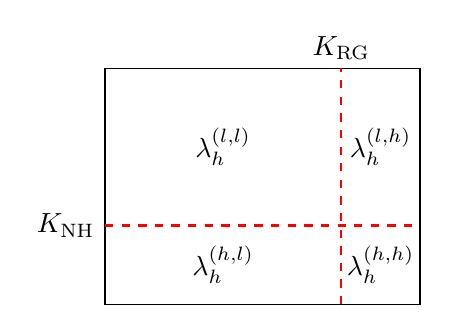
\begin{tikzpicture}
        \draw  (0,0) rectangle (4,3);
        \draw [dashed, red, thick] (0,1) -- (4,1);
        \draw [dashed, red, thick] (3,0) -- (3,3);
        \node at (-.5,1) {$K_{\NH}$};
        \node at (3,3.25) {$K_{\RG}$};
        \node at (1.5,2) {$\lambda_{h}^{(l,l)}$};
        \node at (3.5,2) {$\lambda_{h}^{(l,h)}$};
        \node at (1.5,.5) {$\lambda_{h}^{(h,l)}$};
        \node at (3.5,.5) {$\lambda_{h}^{(h,h)}$};
    \end{tikzpicture}
\caption{General arrival rates for each CCU at each region, where $h\in\{\NH, \RG\}$} \label{arrivalrateregions}
\end{center}
\end{figure}

To formally investigate the impact of decentralised decision making, the interaction between two CCUs is placed within a non-cooperative game framework.
The interaction will be modelled through a two dimensional continuous Markov chain that will now be described.

\subsection{Queueing Model}

The state space for the Markov chain is given by:

\begin{equation}
S=S(c_{\NH}, c_{\RG})= \{(u,v)\in \mathbb{Z}^2\ |\ 0\leq u\leq c_{\NH},\ 0\leq v\leq c_{\RG}\} \label{statespace}
\end{equation}

For given $K_{\NH}, K_{\RG}$ and using the notation of Figure \ref{arrivalrateregions} the generic Markov chain used to model the interactive queueing system in this paper is shown in Figure \ref{mc}.

\begin{figure}[!htbp]
\begin{center}
    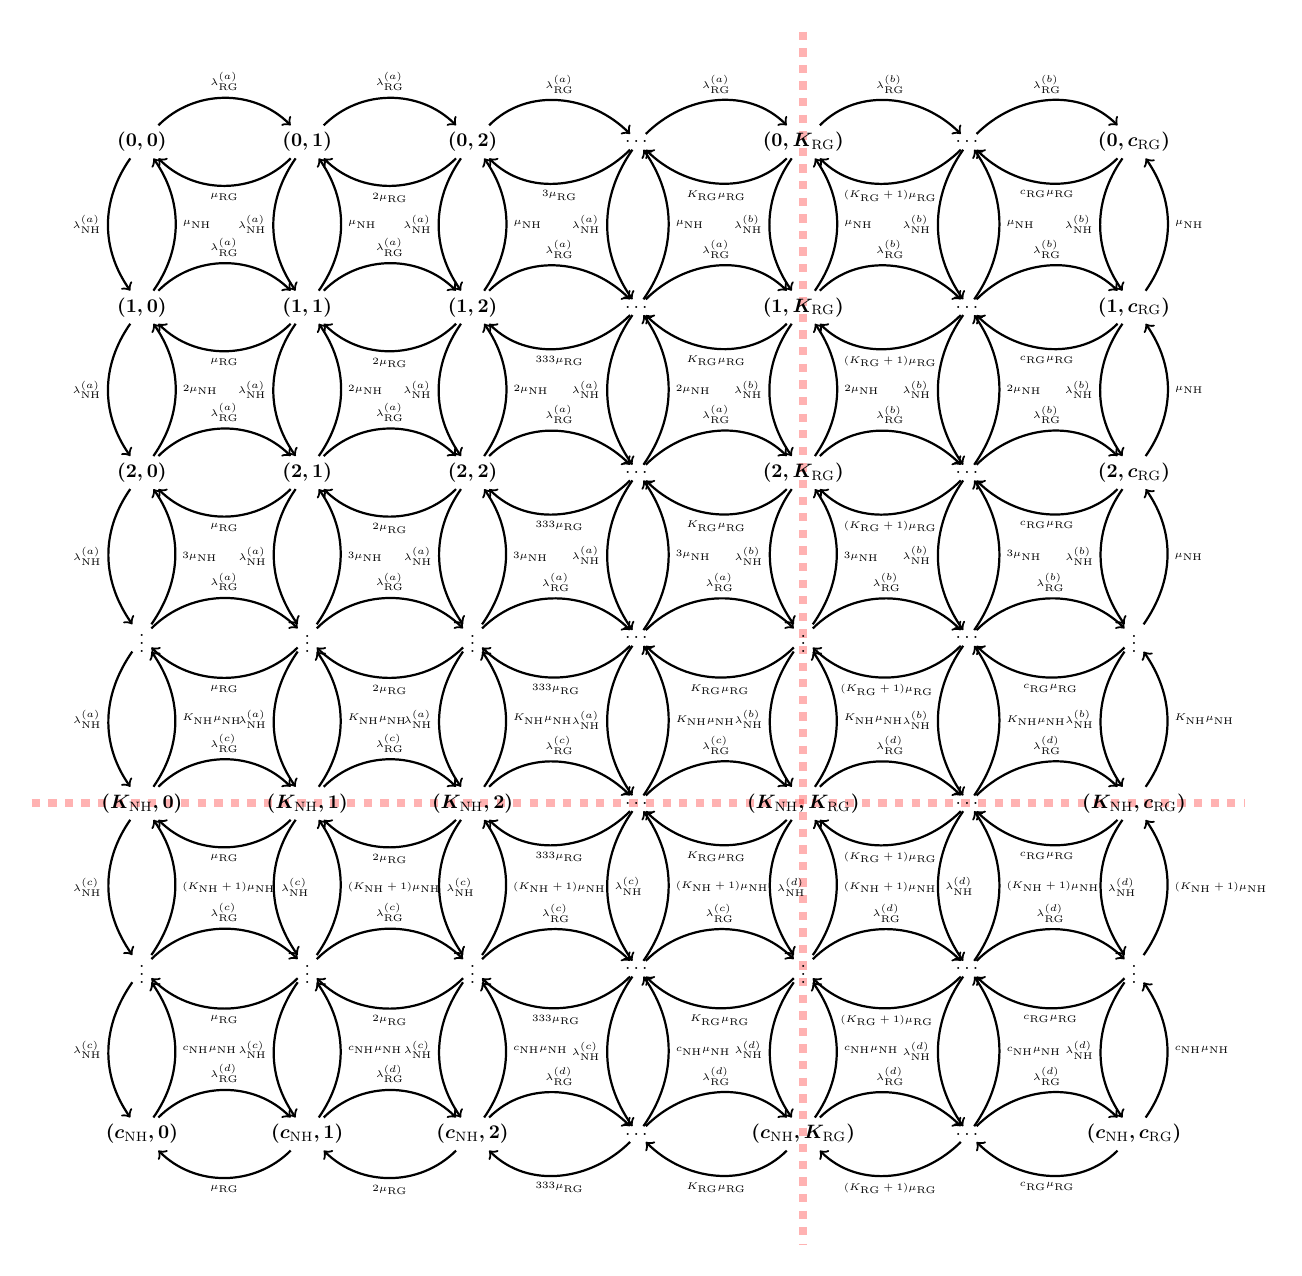
\begin{tikzpicture}[scale=.7, every node/.style={scale=0.7}]
        % -----------------------------------------------
        % Boundaries ------------------------------------
        % -----------------------------------------------
        \draw [dashed, line width=1mm, red, opacity=.3] (12,2) -- (12,-20);
        \draw [dashed, line width=1mm, red, opacity=.3] (-2,-12) -- (20,-12);
        %\tikzstyle{state}=[ellipse, draw, fill=blue!10, minimum width=2cm];
        %\tikzstyle{state}=[rectangle, draw, fill=blue!10, minimum width=2cm];
        \tikzstyle{state}=[minimum width=2cm, font=\boldmath];
        %\draw  (0,0) rectangle (4,3);
        %\draw [dashed, red, thick] (0,1) -- (4,1);
        %\draw [dashed, red, thick] (3,0) -- (3,3);
        % -----------------------------------------------
        % First row--------------------------------------
        % -----------------------------------------------
        \node (aa) [state] at (0,0) {$(0,0)$};
        \node (ab) [state] at ($(aa) + (3,0)$) {$(0,1)$};
        \node (ac) [state] at ($(ab) + (3,0)$) {$(0,2)$};
        \node (ellipsisa1) at ($(ac) + (3,0)$) {$\dots$};
        \node(ak) [state] at ($(ellipsisa1) + (3,0)$) {$(0,K_{\RG})$};
        \node (ellipsisa2) at ($(ak) + (3,0)$) {$\dots$};
        \node(az) [state] at ($(ellipsisa2) + (3,0)$) {$(0,c_{\RG})$};
        % Transitions -----------------------------------
        % On Row:
        \draw (aa) edge[out=45,in=135,->,thick] node [above] {\tiny$\lambda_{\RG}^{(a)}$} (ab);
        \draw (aa) edge[out=-45,in=-135,<-,thick] node [below] {\tiny$\mu_{\RG}$} (ab);

        \draw (ab) edge[out=45,in=135,->,thick] node [above] {\tiny$\lambda_{\RG}^{(a)}$} (ac);
        \draw (ab) edge[out=-45,in=-135,<-,thick] node [below] {\tiny$2\mu_{\RG}$} (ac);

        \draw (ac) edge[out=45,in=135,->,thick] node [above] {\tiny$\lambda_{\RG}^{(a)}$} (ellipsisa1);
        \draw (ac) edge[out=-45,in=-135,<-,thick] node [below] {\tiny$3\mu_{\RG}$} (ellipsisa1);

        \draw (ellipsisa1) edge[out=45,in=135,->,thick] node [above] {\tiny$\lambda_{\RG}^{(a)}$} (ak);
        \draw (ellipsisa1) edge[out=-45,in=-135,<-,thick] node [below] {\tiny$K_{\RG}\mu_{\RG}$} (ak);

        \draw (ak) edge[out=45,in=135,->,thick] node [above] {\tiny$\lambda_{\RG}^{(b)}$} (ellipsisa2);
        \draw (ak) edge[out=-45,in=-135,<-,thick] node [below] {\tiny$(K_{\RG}+1)\mu_{\RG}$} (ellipsisa2);

        \draw (ellipsisa2) edge[out=45,in=135,->,thick] node [above] {\tiny$\lambda_{\RG}^{(b)}$} (az);
        \draw (ellipsisa2) edge[out=-45,in=-135,<-,thick] node [below] {\tiny$c_{\RG}\mu_{\RG}$} (az);
        % -----------------------------------------------
        % Second row--------------------------------------
        % -----------------------------------------------
        \node (ba) [state] at (0,-3) {$(1,0)$};
        \node (bb) [state] at ($(ba) + (3,0)$) {$(1,1)$};
        \node (bc) [state] at ($(bb) + (3,0)$) {$(1,2)$};
        \node (ellipsisb1) at ($(bc) + (3,0)$) {$\dots$};
        \node(bk) [state] at ($(ellipsisb1) + (3,0)$) {$(1,K_{\RG})$};
        \node (ellipsisb2) at ($(bk) + (3,0)$) {$\dots$};
        \node(bz) [state] at ($(ellipsisb2) + (3,0)$) {$(1,c_{\RG})$};
        % Transitions -----------------------------------
        % On Row:
        \draw (ba) edge[out=45,in=135,->,thick] node [above] {\tiny$\lambda_{\RG}^{(a)}$} (bb);
        \draw (ba) edge[out=-45,in=-135,<-,thick] node [below] {\tiny$\mu_{\RG}$} (bb);

        \draw (bb) edge[out=45,in=135,->,thick] node [above] {\tiny$\lambda_{\RG}^{(a)}$} (bc);
        \draw (bb) edge[out=-45,in=-135,<-,thick] node [below] {\tiny$2\mu_{\RG}$} (bc);

        \draw (bc) edge[out=45,in=135,->,thick] node [above] {\tiny$\lambda_{\RG}^{(a)}$} (ellipsisb1);
        \draw (bc) edge[out=-45,in=-135,<-,thick] node [below] {\tiny$333\mu_{\RG}$} (ellipsisb1);

        \draw (ellipsisb1) edge[out=45,in=135,->,thick] node [above] {\tiny$\lambda_{\RG}^{(a)}$} (bk);
        \draw (ellipsisb1) edge[out=-45,in=-135,<-,thick] node [below] {\tiny$K_{\RG}\mu_{\RG}$} (bk);

        \draw (bk) edge[out=45,in=135,->,thick] node [above] {\tiny$\lambda_{\RG}^{(b)}$} (ellipsisb2);
        \draw (bk) edge[out=-45,in=-135,<-,thick] node [below] {\tiny$(K_{\RG} + 1)\mu_{\RG}$} (ellipsisb2);

        \draw (ellipsisb2) edge[out=45,in=135,->,thick] node [above] {\tiny$\lambda_{\RG}^{(b)}$} (bz);
        \draw (ellipsisb2) edge[out=-45,in=-135,<-,thick] node [below] {\tiny$c_{\RG}\mu_{\RG}$} (bz);
        % With previous row:
        \draw (aa) edge[out=-125,in=125,->,thick] node [left] {\tiny$\lambda_{\NH}^{(a)}$} (ba);
        \draw (aa) edge[out=-55,in=55,<-,thick] node [right] {\tiny$\mu_{\NH}$} (ba);

        \draw (ab) edge[out=-125,in=125,->,thick] node [left] {\tiny$\lambda_{\NH}^{(a)}$} (bb);
        \draw (ab) edge[out=-55,in=55,<-,thick] node [right] {\tiny$\mu_{\NH}$} (bb);

        \draw (ac) edge[out=-125,in=125,->,thick] node [left] {\tiny$\lambda_{\NH}^{(a)}$} (bc);
        \draw (ac) edge[out=-55,in=55,<-,thick] node [right] {\tiny$\mu_{\NH}$} (bc);

        \draw (ellipsisa1) edge[out=-125,in=125,->,thick] node [left] {\tiny$\lambda_{\NH}^{(a)}$} (ellipsisb1);
        \draw (ellipsisa1) edge[out=-55,in=55,<-,thick] node [right] {\tiny$\mu_{\NH}$} (ellipsisb1);

        \draw (ak) edge[out=-125,in=125,->,thick] node [left] {\tiny$\lambda_{\NH}^{(b)}$} (bk);
        \draw (ak) edge[out=-55,in=55,<-,thick] node [right] {\tiny$\mu_{\NH}$} (bk);

        \draw (ellipsisa2) edge[out=-125,in=125,->,thick] node [left] {\tiny$\lambda_{\NH}^{(b)}$} (ellipsisb2);
        \draw (ellipsisa2) edge[out=-55,in=55,<-,thick] node [right] {\tiny$\mu_{\NH}$} (ellipsisb2);

        \draw (az) edge[out=-125,in=125,->,thick] node [left] {\tiny$\lambda_{\NH}^{(b)}$} (bz);
        \draw (az) edge[out=-55,in=55,<-,thick] node [right] {\tiny$\mu_{\NH}$} (bz);
        % -----------------------------------------------
        % Third row--------------------------------------
        % -----------------------------------------------
        \node (ca) [state] at (0,-6) {$(2,0)$};
        \node (cb) [state] at ($(ca) + (3,0)$) {$(2,1)$};
        \node (cc) [state] at ($(cb) + (3,0)$) {$(2,2)$};
        \node (ellipsisc1) at ($(cc) + (3,0)$) {$\dots$};
        \node(ck) [state] at ($(ellipsisc1) + (3,0)$) {$(2,K_{\RG})$};
        \node (ellipsisc2) at ($(ck) + (3,0)$) {$\dots$};
        \node(cz) [state] at ($(ellipsisc2) + (3,0)$) {$(2,c_{\RG})$};
        % Transitions -----------------------------------
        % On Row:
        \draw (ca) edge[out=45,in=135,->,thick] node [above] {\tiny$\lambda_{\RG}^{(a)}$} (cb);
        \draw (ca) edge[out=-45,in=-135,<-,thick] node [below] {\tiny$\mu_{\RG}$} (cb);

        \draw (cb) edge[out=45,in=135,->,thick] node [above] {\tiny$\lambda_{\RG}^{(a)}$} (cc);
        \draw (cb) edge[out=-45,in=-135,<-,thick] node [below] {\tiny$2\mu_{\RG}$} (cc);

        \draw (cc) edge[out=45,in=135,->,thick] node [above] {\tiny$\lambda_{\RG}^{(a)}$} (ellipsisc1);
        \draw (cc) edge[out=-45,in=-135,<-,thick] node [below] {\tiny$333\mu_{\RG}$} (ellipsisc1);

        \draw (ellipsisc1) edge[out=45,in=135,->,thick] node [above] {\tiny$\lambda_{\RG}^{(a)}$} (ck);
        \draw (ellipsisc1) edge[out=-45,in=-135,<-,thick] node [below] {\tiny$K_{\RG}\mu_{\RG}$} (ck);

        \draw (ck) edge[out=45,in=135,->,thick] node [above] {\tiny$\lambda_{\RG}^{(b)}$} (ellipsisc2);
        \draw (ck) edge[out=-45,in=-135,<-,thick] node [below] {\tiny$(K_{\RG} + 1)\mu_{\RG}$} (ellipsisc2);

        \draw (ellipsisc2) edge[out=45,in=135,->,thick] node [above] {\tiny$\lambda_{\RG}^{(b)}$} (cz);
        \draw (ellipsisc2) edge[out=-45,in=-135,<-,thick] node [below] {\tiny$c_{\RG}\mu_{\RG}$} (cz);
        % With previous row:
        \draw (ba) edge[out=-125,in=125,->,thick] node [left] {\tiny$\lambda_{\NH}^{(a)}$} (ca);
        \draw (ba) edge[out=-55,in=55,<-,thick] node [right] {\tiny$2\mu_{\NH}$} (ca);

        \draw (bb) edge[out=-125,in=125,->,thick] node [left] {\tiny$\lambda_{\NH}^{(a)}$} (cb);
        \draw (bb) edge[out=-55,in=55,<-,thick] node [right] {\tiny$2\mu_{\NH}$} (cb);

        \draw (bc) edge[out=-125,in=125,->,thick] node [left] {\tiny$\lambda_{\NH}^{(a)}$} (cc);
        \draw (bc) edge[out=-55,in=55,<-,thick] node [right] {\tiny$2\mu_{\NH}$} (cc);

        \draw (ellipsisb1) edge[out=-125,in=125,->,thick] node [left] {\tiny$\lambda_{\NH}^{(a)}$} (ellipsisc1);
        \draw (ellipsisb1) edge[out=-55,in=55,<-,thick] node [right] {\tiny$2\mu_{\NH}$} (ellipsisc1);

        \draw (bk) edge[out=-125,in=125,->,thick] node [left] {\tiny$\lambda_{\NH}^{(b)}$} (ck);
        \draw (bk) edge[out=-55,in=55,<-,thick] node [right] {\tiny$2\mu_{\NH}$} (ck);

        \draw (ellipsisb2) edge[out=-125,in=125,->,thick] node [left] {\tiny$\lambda_{\NH}^{(b)}$} (ellipsisc2);
        \draw (ellipsisb2) edge[out=-55,in=55,<-,thick] node [right] {\tiny$2\mu_{\NH}$} (ellipsisc2);

        \draw (bz) edge[out=-125,in=125,->,thick] node [left] {\tiny$\lambda_{\NH}^{(b)}$} (cz);
        \draw (bz) edge[out=-55,in=55,<-,thick] node [right] {\tiny$\mu_{\NH}$} (cz);
        % -----------------------------------------------
        % Fourth row--------------------------------------
        % -----------------------------------------------
        \node (da) at (0,-9) {$\vdots$};
        \node (db) at ($(da) + (3,0)$) {$\vdots$};
        \node (dc) at ($(db) + (3,0)$) {$\vdots$};
        \node (ellipsisd1) at ($(dc) + (3,0)$) {$\dots$};
        \node(dk) at ($(ellipsisd1) + (3,0)$) {$\vdots$};
        \node (ellipsisd2) at ($(dk) + (3,0)$) {$\dots$};
        \node(dz) at ($(ellipsisd2) + (3,0)$) {$\vdots$};
        % Transitions -----------------------------------
        % On Row:
        \draw (da) edge[out=45,in=135,->,thick] node [above] {\tiny$\lambda_{\RG}^{(a)}$} (db);
        \draw (da) edge[out=-45,in=-135,<-,thick] node [below] {\tiny$\mu_{\RG}$} (db);

        \draw (db) edge[out=45,in=135,->,thick] node [above] {\tiny$\lambda_{\RG}^{(a)}$} (dc);
        \draw (db) edge[out=-45,in=-135,<-,thick] node [below] {\tiny$2\mu_{\RG}$} (dc);

        \draw (dc) edge[out=45,in=135,->,thick] node [above] {\tiny$\lambda_{\RG}^{(a)}$} (ellipsisd1);
        \draw (dc) edge[out=-45,in=-135,<-,thick] node [below] {\tiny$333\mu_{\RG}$} (ellipsisd1);

        \draw (ellipsisd1) edge[out=45,in=135,->,thick] node [above] {\tiny$\lambda_{\RG}^{(a)}$} (dk);
        \draw (ellipsisd1) edge[out=-45,in=-135,<-,thick] node [below] {\tiny$K_{\RG}\mu_{\RG}$} (dk);

        \draw (dk) edge[out=45,in=135,->,thick] node [above] {\tiny$\lambda_{\RG}^{(b)}$} (ellipsisd2);
        \draw (dk) edge[out=-45,in=-135,<-,thick] node [below] {\tiny$(K_{\RG} + 1)\mu_{\RG}$} (ellipsisd2);

        \draw (ellipsisd2) edge[out=45,in=135,->,thick] node [above] {\tiny$\lambda_{\RG}^{(b)}$} (dz);
        \draw (ellipsisd2) edge[out=-45,in=-135,<-,thick] node [below] {\tiny$c_{\RG}\mu_{\RG}$} (dz);
        % With previous row:
        \draw (ca) edge[out=-125,in=125,->,thick] node [left] {\tiny$\lambda_{\NH}^{(a)}$} (da);
        \draw (ca) edge[out=-55,in=55,<-,thick] node [right] {\tiny$3\mu_{\NH}$} (da);

        \draw (cb) edge[out=-125,in=125,->,thick] node [left] {\tiny$\lambda_{\NH}^{(a)}$} (db);
        \draw (cb) edge[out=-55,in=55,<-,thick] node [right] {\tiny$3\mu_{\NH}$} (db);

        \draw (cc) edge[out=-125,in=125,->,thick] node [left] {\tiny$\lambda_{\NH}^{(a)}$} (dc);
        \draw (cc) edge[out=-55,in=55,<-,thick] node [right] {\tiny$3\mu_{\NH}$} (dc);

        \draw (ellipsisc1) edge[out=-125,in=125,->,thick] node [left] {\tiny$\lambda_{\NH}^{(a)}$} (ellipsisd1);
        \draw (ellipsisc1) edge[out=-55,in=55,<-,thick] node [right] {\tiny$3\mu_{\NH}$} (ellipsisd1);

        \draw (ck) edge[out=-125,in=125,->,thick] node [left] {\tiny$\lambda_{\NH}^{(b)}$} (dk);
        \draw (ck) edge[out=-55,in=55,<-,thick] node [right] {\tiny$3\mu_{\NH}$} (dk);

        \draw (ellipsisc2) edge[out=-125,in=125,->,thick] node [left] {\tiny$\lambda_{\NH}^{(b)}$} (ellipsisd2);
        \draw (ellipsisc2) edge[out=-55,in=55,<-,thick] node [right] {\tiny$3\mu_{\NH}$} (ellipsisd2);

        \draw (cz) edge[out=-125,in=125,->,thick] node [left] {\tiny$\lambda_{\NH}^{(b)}$} (dz);
        \draw (cz) edge[out=-55,in=55,<-,thick] node [right] {\tiny$\mu_{\NH}$} (dz);
        % -----------------------------------------------
        % Fifth row--------------------------------------
        % -----------------------------------------------
        \node (ea) [state] at (0,-12) {$(K_{\NH},0)$};
        \node (eb) [state] at ($(ea) + (3,0)$) {$(K_{\NH},1)$};
        \node (ec) [state] at ($(eb) + (3,0)$) {$(K_{\NH},2)$};
        \node (ellipsise1) at ($(ec) + (3,0)$) {$\dots$};
        \node(ek) [state] at ($(ellipsise1) + (3,0)$) {$(K_{\NH},K_{\RG})$};
        \node (ellipsise2) at ($(ek) + (3,0)$) {$\dots$};
        \node(ez) [state] at ($(ellipsise2) + (3,0)$) {$(K_{\NH},c_{\RG})$};
        % Transitions -----------------------------------
        % On Row:
        \draw (ea) edge[out=45,in=135,->,thick] node [above] {\tiny$\lambda_{\RG}^{(c)}$} (eb);
        \draw (ea) edge[out=-45,in=-135,<-,thick] node [below] {\tiny$\mu_{\RG}$} (eb);

        \draw (eb) edge[out=45,in=135,->,thick] node [above] {\tiny$\lambda_{\RG}^{(c)}$} (ec);
        \draw (eb) edge[out=-45,in=-135,<-,thick] node [below] {\tiny$2\mu_{\RG}$} (ec);

        \draw (ec) edge[out=45,in=135,->,thick] node [above] {\tiny$\lambda_{\RG}^{(c)}$} (ellipsise1);
        \draw (ec) edge[out=-45,in=-135,<-,thick] node [below] {\tiny$333\mu_{\RG}$} (ellipsise1);

        \draw (ellipsise1) edge[out=45,in=135,->,thick] node [above] {\tiny$\lambda_{\RG}^{(c)}$} (ek);
        \draw (ellipsise1) edge[out=-45,in=-135,<-,thick] node [below] {\tiny$K_{\RG}\mu_{\RG}$} (ek);

        \draw (ek) edge[out=45,in=135,->,thick] node [above] {\tiny$\lambda_{\RG}^{(d)}$} (ellipsise2);
        \draw (ek) edge[out=-45,in=-135,<-,thick] node [below] {\tiny$(K_{\RG} + 1)\mu_{\RG}$} (ellipsise2);

        \draw (ellipsise2) edge[out=45,in=135,->,thick] node [above] {\tiny$\lambda_{\RG}^{(d)}$} (ez);
        \draw (ellipsise2) edge[out=-45,in=-135,<-,thick] node [below] {\tiny$c_{\RG}\mu_{\RG}$} (ez);
        % With previous row:
        \draw (da) edge[out=-125,in=125,->,thick] node [left] {\tiny$\lambda_{\NH}^{(a)}$} (ea);
        \draw (da) edge[out=-55,in=55,<-,thick] node [right] {\tiny$K_{\NH}\mu_{\NH}$} (ea);

        \draw (db) edge[out=-125,in=125,->,thick] node [left] {\tiny$\lambda_{\NH}^{(a)}$} (eb);
        \draw (db) edge[out=-55,in=55,<-,thick] node [right] {\tiny$K_{\NH}\mu_{\NH}$} (eb);

        \draw (dc) edge[out=-125,in=125,->,thick] node [left] {\tiny$\lambda_{\NH}^{(a)}$} (ec);
        \draw (dc) edge[out=-55,in=55,<-,thick] node [right] {\tiny$K_{\NH}\mu_{\NH}$} (ec);

        \draw (ellipsisd1) edge[out=-125,in=125,->,thick] node [left] {\tiny$\lambda_{\NH}^{(a)}$} (ellipsise1);
        \draw (ellipsisd1) edge[out=-55,in=55,<-,thick] node [right] {\tiny$K_{\NH}\mu_{\NH}$} (ellipsise1);

        \draw (dk) edge[out=-125,in=125,->,thick] node [left] {\tiny$\lambda_{\NH}^{(b)}$} (ek);
        \draw (dk) edge[out=-55,in=55,<-,thick] node [right] {\tiny$K_{\NH}\mu_{\NH}$} (ek);

        \draw (ellipsisd2) edge[out=-125,in=125,->,thick] node [left] {\tiny$\lambda_{\NH}^{(b)}$} (ellipsise2);
        \draw (ellipsisd2) edge[out=-55,in=55,<-,thick] node [right] {\tiny$K_{\NH}\mu_{\NH}$} (ellipsise2);

        \draw (dz) edge[out=-125,in=125,->,thick] node [left] {\tiny$\lambda_{\NH}^{(b)}$} (ez);
        \draw (dz) edge[out=-55,in=55,<-,thick] node [right] {\tiny$K_{\NH}\mu_{\NH}$} (ez);
        % Sixth row--------------------------------------
        \node (fa) at (0,-15) {$\vdots$};
        \node (fb) at ($(fa) + (3,0)$) {$\vdots$};
        \node (fc) at ($(fb) + (3,0)$) {$\vdots$};
        \node (ellipsisf1) at ($(fc) + (3,0)$) {$\dots$};
        \node(fk) at ($(ellipsisf1) + (3,0)$) {$\vdots$};
        \node (ellipsisf2) at ($(fk) + (3,0)$) {$\dots$};
        \node(fz) at ($(ellipsisf2) + (3,0)$) {$\vdots$};
        % Transitions -----------------------------------
        % On Row:
        \draw (fa) edge[out=45,in=135,->,thick] node [above] {\tiny$\lambda_{\RG}^{(c)}$} (fb);
        \draw (fa) edge[out=-45,in=-135,<-,thick] node [below] {\tiny$\mu_{\RG}$} (fb);

        \draw (fb) edge[out=45,in=135,->,thick] node [above] {\tiny$\lambda_{\RG}^{(c)}$} (fc);
        \draw (fb) edge[out=-45,in=-135,<-,thick] node [below] {\tiny$2\mu_{\RG}$} (fc);

        \draw (fc) edge[out=45,in=135,->,thick] node [above] {\tiny$\lambda_{\RG}^{(c)}$} (ellipsisf1);
        \draw (fc) edge[out=-45,in=-135,<-,thick] node [below] {\tiny$333\mu_{\RG}$} (ellipsisf1);

        \draw (ellipsisf1) edge[out=45,in=135,->,thick] node [above] {\tiny$\lambda_{\RG}^{(c)}$} (fk);
        \draw (ellipsisf1) edge[out=-45,in=-135,<-,thick] node [below] {\tiny$K_{\RG}\mu_{\RG}$} (fk);

        \draw (fk) edge[out=45,in=135,->,thick] node [above] {\tiny$\lambda_{\RG}^{(d)}$} (ellipsisf2);
        \draw (fk) edge[out=-45,in=-135,<-,thick] node [below] {\tiny$(K_{\RG} + 1)\mu_{\RG}$} (ellipsisf2);

        \draw (ellipsisf2) edge[out=45,in=135,->,thick] node [above] {\tiny$\lambda_{\RG}^{(d)}$} (fz);
        \draw (ellipsisf2) edge[out=-45,in=-135,<-,thick] node [below] {\tiny$c_{\RG}\mu_{\RG}$} (fz);
        % With previous row:
        \draw (ea) edge[out=-125,in=125,->,thick] node [left] {\tiny$\lambda_{\NH}^{(c)}$} (fa);
        \draw (ea) edge[out=-55,in=55,<-,thick] node [right] {\tiny$(K_{\NH}+1)\mu_{\NH}$} (fa);

        \draw (eb) edge[out=-125,in=125,->,thick] node [right] {\tiny$\lambda_{\NH}^{(c)}$} (fb);
        \draw (eb) edge[out=-55,in=55,<-,thick] node [right] {\tiny$(K_{\NH} + 1)\mu_{\NH}$} (fb);

        \draw (ec) edge[out=-125,in=125,->,thick] node [right] {\tiny$\lambda_{\NH}^{(c)}$} (fc);
        \draw (ec) edge[out=-55,in=55,<-,thick] node [right] {\tiny$(K_{\NH} + 1)\mu_{\NH}$} (fc);

        \draw (ellipsise1) edge[out=-125,in=125,->,thick] node [right] {\tiny$\lambda_{\NH}^{(c)}$} (ellipsisf1);
        \draw (ellipsise1) edge[out=-55,in=55,<-,thick] node [right] {\tiny$(K_{\NH} + 1)\mu_{\NH}$} (ellipsisf1);

        \draw (ek) edge[out=-125,in=125,->,thick] node [right] {\tiny$\lambda_{\NH}^{(d)}$} (fk);
        \draw (ek) edge[out=-55,in=55,<-,thick] node [right] {\tiny$(K_{\NH} + 1)\mu_{\NH}$} (fk);

        \draw (ellipsise2) edge[out=-125,in=125,->,thick] node [right] {\tiny$\lambda_{\NH}^{(d)}$} (ellipsisf2);
        \draw (ellipsise2) edge[out=-55,in=55,<-,thick] node [right] {\tiny$(K_{\NH} + 1)\mu_{\NH}$} (ellipsisf2);

        \draw (ez) edge[out=-125,in=125,->,thick] node [right] {\tiny$\lambda_{\NH}^{(d)}$} (fz);
        \draw (ez) edge[out=-55,in=55,<-,thick] node [right] {\tiny$(K_{\NH}+1)\mu_{\NH}$} (fz);
        % Final row--------------------------------------
        \node (za) [state] at (0,-18) {$(c_{\NH},0)$};
        \node (zb) [state] at ($(za) + (3,0)$) {$(c_{\NH},1)$};
        \node (zc) [state] at ($(zb) + (3,0)$) {$(c_{\NH},2)$};
        \node (ellipsisz1) at ($(zc) + (3,0)$) {$\dots$};
        \node(zk) [state] at ($(ellipsisz1) + (3,0)$) {$(c_{\NH},K_{\RG})$};
        \node (ellipsisz2) at ($(zk) + (3,0)$) {$\dots$};
        \node(zz) [state] at ($(ellipsisz2) + (3,0)$) {$(c_{\NH},c_{\RG})$};
        % Transitions -----------------------------------
        % On Row:
        \draw (za) edge[out=45,in=135,->,thick] node [above] {\tiny$\lambda_{\RG}^{(d)}$} (zb);
        \draw (za) edge[out=-45,in=-135,<-,thick] node [below] {\tiny$\mu_{\RG}$} (zb);

        \draw (zb) edge[out=45,in=135,->,thick] node [above] {\tiny$\lambda_{\RG}^{(d)}$} (zc);
        \draw (zb) edge[out=-45,in=-135,<-,thick] node [below] {\tiny$2\mu_{\RG}$} (zc);

        \draw (zc) edge[out=45,in=135,->,thick] node [above] {\tiny$\lambda_{\RG}^{(d)}$} (ellipsisz1);
        \draw (zc) edge[out=-45,in=-135,<-,thick] node [below] {\tiny$333\mu_{\RG}$} (ellipsisz1);

        \draw (ellipsisz1) edge[out=45,in=135,->,thick] node [above] {\tiny$\lambda_{\RG}^{(d)}$} (zk);
        \draw (ellipsisz1) edge[out=-45,in=-135,<-,thick] node [below] {\tiny$K_{\RG}\mu_{\RG}$} (zk);

        \draw (zk) edge[out=45,in=135,->,thick] node [above] {\tiny$\lambda_{\RG}^{(d)}$} (ellipsisz2);
        \draw (zk) edge[out=-45,in=-135,<-,thick] node [below] {\tiny$(K_{\RG} + 1)\mu_{\RG}$} (ellipsisz2);

        \draw (ellipsisz2) edge[out=45,in=135,->,thick] node [above] {\tiny$\lambda_{\RG}^{(d)}$} (zz);
        \draw (ellipsisz2) edge[out=-45,in=-135,<-,thick] node [below] {\tiny$c_{\RG}\mu_{\RG}$} (zz);
        % With previous row:
        \draw (fa) edge[out=-125,in=125,->,thick] node [left] {\tiny$\lambda_{\NH}^{(c)}$} (za);
        \draw (fa) edge[out=-55,in=55,<-,thick] node [right] {\tiny$c_{\NH}\mu_{\NH}$} (za);

        \draw (fb) edge[out=-125,in=125,->,thick] node [left] {\tiny$\lambda_{\NH}^{(c)}$} (zb);
        \draw (fb) edge[out=-55,in=55,<-,thick] node [right] {\tiny$c_{\NH}\mu_{\NH}$} (zb);

        \draw (fc) edge[out=-125,in=125,->,thick] node [left] {\tiny$\lambda_{\NH}^{(c)}$} (zc);
        \draw (fc) edge[out=-55,in=55,<-,thick] node [right] {\tiny$c_{\NH}\mu_{\NH}$} (zc);

        \draw (ellipsisf1) edge[out=-125,in=125,->,thick] node [left] {\tiny$\lambda_{\NH}^{(c)}$} (ellipsisz1);
        \draw (ellipsisf1) edge[out=-55,in=55,<-,thick] node [right] {\tiny$c_{\NH}\mu_{\NH}$} (ellipsisz1);

        \draw (fk) edge[out=-125,in=125,->,thick] node [left] {\tiny$\lambda_{\NH}^{(d)}$} (zk);
        \draw (fk) edge[out=-55,in=55,<-,thick] node [right] {\tiny$c_{\NH}\mu_{\NH}$} (zk);

        \draw (ellipsisf2) edge[out=-125,in=125,->,thick] node [left] {\tiny$\lambda_{\NH}^{(d)}$} (ellipsisz2);
        \draw (ellipsisf2) edge[out=-55,in=55,<-,thick] node [right] {\tiny$c_{\NH}\mu_{\NH}$} (ellipsisz2);

        \draw (fz) edge[out=-125,in=125,->,thick] node [left] {\tiny$\lambda_{\NH}^{(d)}$} (zz);
        \draw (fz) edge[out=-55,in=55,<-,thick] node [right] {\tiny$c_{\NH}\mu_{\NH}$} (zz);

    \end{tikzpicture}
\caption{Generic Markov chain underpinning the queueing model of this paper} \label{mc}
\end{center}
\end{figure}

In total there are $(c_{\NH}+1)\times(c_{\RG}+1)$ states and they are indexed lexicographically: $(0,0), (0,1), (0,2)$, etc. In general, state $(u,v)$ is the $s(u,v)th$ state where $s(u,v)=u(c_{\RG}+1)+(v+1)$.

The stochastic transition rate matrix $Q=Q(c_{NH},c_{RG})$ of the continuous-time Markov chain \cite{Stewart2009} has entries $q_{ij}$ which is the rate at which a transition from state $i$ to state $j$ occurs. The transition rates are given by:

\begin{equation}
q_{ij}=\begin{cases} u\mu_{\NH} & \text{ if  } (u_i,v_i)-(u_j,v_j)=(1,0),\\
 v\mu_{\RG} & \text{ if  } (u_i,v_i)-(u_j,v_j)=(0,1),\\
 \lambda_{NH}^{(a)} & \text{ if  } (u_i,v_i)-(u_j,v_j)=(-1,0)  \text{ and  } u_i < K_{\NH}  \text{ and  } v_i < K_{\RG},\\
 \lambda_{RG}^{(a)} & \text{ if  } (u_i,v_i)-(u_j,v_j)=(0,-1)  \text{ and  } u_i < K_{\NH}  \text{ and  } v_i < K_{\RG},\\
\lambda_{NH}^{(b)} & \text{ if  } (u_i,v_i)-(u_j,v_j)=(-1,0) \text{ and  } u_i < K_{\NH}  \text{ and  } v_i \geq K_{\RG},\\
\lambda_{RG}^{(b)} & \text{ if  } (u_i,v_i)-(u_j,v_j)=(0,-1) \text{ and  } u_i < K_{\NH}  \text{ and  } v_i \geq K_{\RG},\\
\lambda_{NH}^{(c)} & \text{ if  } (u_i,v_i)-(u_j,v_j)=(-1,0) \text{ and  } u_i \geq K_{\NH}  \text{ and  } v_i < K_{\RG},\\
\lambda_{RG}^{(c)} & \text{ if  } (u_i,v_i)-(u_j,v_j)=(0,-1) \text{ and  } u_i \geq K_{\NH}  \text{ and  } v_i < K_{\RG},\\
\lambda_{NH}^{(d)} & \text{ if  } (u_i,v_i)-(u_j,v_j)=(-1,0) \text{ and  } u_i \geq K_{\NH}  \text{ and  } v_i \geq K_{\RG},\\
\lambda_{RG}^{(d)} & \text{ if  } (u_i,v_i)-(u_j,v_j)=(0,-1) \text{ and  } u_i \geq K_{\NH}  \text{ and  } v_i \geq K_{\RG},\\
0 & \text{ otherwise}.
\end{cases}
\end{equation}

Utilities will be of interest when this queueing theoretical model will be inserted in the game theoretical model.
Throughput of patients is a natural choice of utility given that most hospitals are financially rewarded per served patient \cite{Pate2009}.
For each threshold pair $(K_{\NH},K_{\RG})$, the utilisation rate $U_h$ and throughput $T_h$ can easily be obtained for each CCU: $h\in\{\text{NH},\text{RG}\}$, using the following formulas:

$$U_{h}={{\sum_{n=0}^{c_h} nP^{(h)}(n)}\over{c_{h}}}$$
$$T_{h}=\mu_h \sum _{n=0}^{c_h} nP^{(h)}(n)$$

where $P^{(h)}=P^{(h)}(K_{\NH},K_{\RG})$ is the steady state probability distribution function (obtained from the corresponding transition matrix $Q=Q(K_{\NH},K_{\RG})$) for $h\in\{\text{NH},\text{RG}\}$.

For $c_{\NH}=8$, $c_{\RG}=16$, $\lambda_{\NH}=(\lambda_{\NH}^{(a)},\lambda_{\NH}^{(b)},\lambda_{\NH}^{(c)},\lambda_{\NH}^{(d)})=(1.5,3.74,0,0)$, $\lambda_{\RG}=(\lambda_{\RG}^{(a)},\lambda_{\RG}^{(b)},\lambda_{\RG}^{(c)},\lambda_{\RG}^{(d)})=(2.24,0,3.74,0)$ and $(K_{\NH},K_{\RG})=(6,12)$, the steady state probabilities for each CCU are given in Figure \ref{steady_state_probs}.

\begin{figure}[!htbp]
$$
\begin{array}{cc}
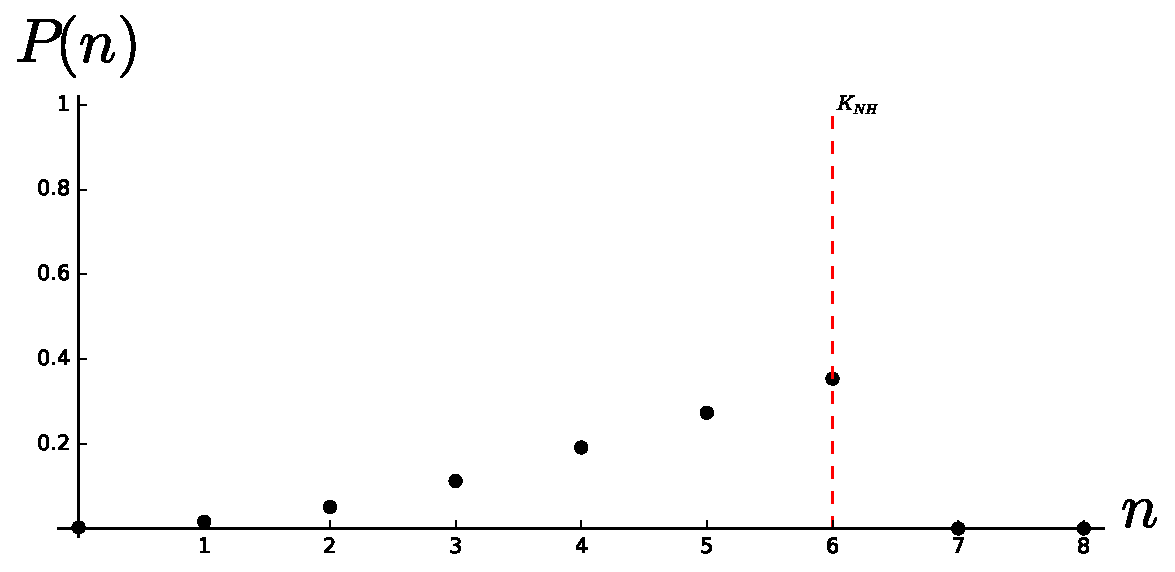
\includegraphics[width=.5\textwidth]{./Images/NH.pdf}&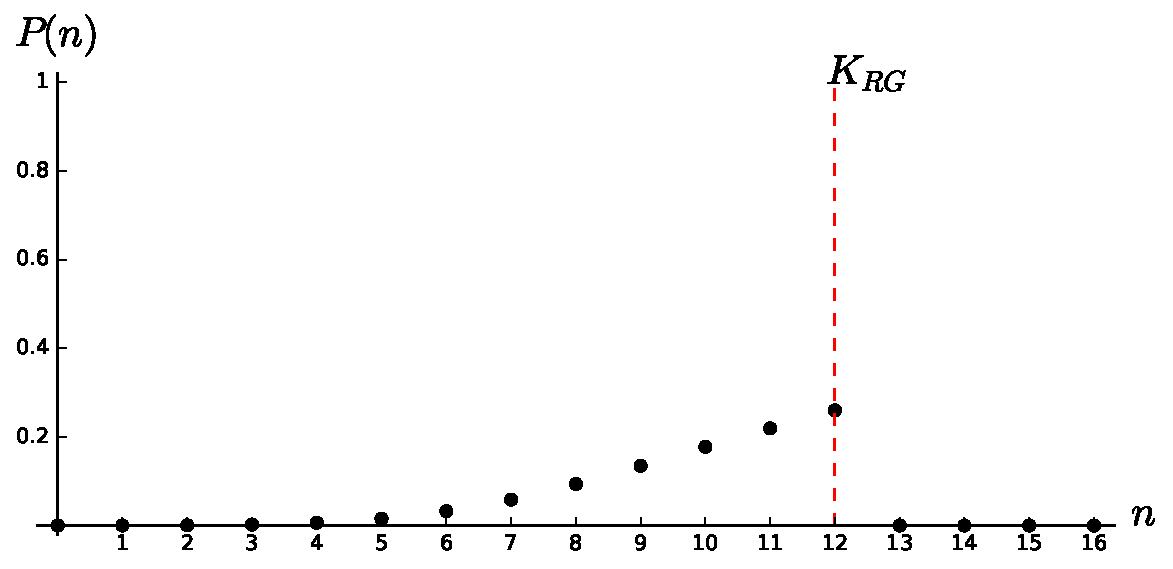
\includegraphics[width=.5\textwidth]{./Images/RG.pdf}\\
h=NH&h=RG
\end{array}
$$
\caption{Steady state probabilities for $h\in\{\NH,\RG\}$ with $(K_{\NH}, K_{\RG})=(6,12)$} \label{steady_state_probs}
\end{figure}

For the parameters of Figure \ref{steady_state_probs} the utilisation rates are: 59\% at NH and 62\% at RG and a throughput of 1.23 at NH and 1.98 at RG (patients per day).\\

For a different threshold pair of $(K_{\NH},K_{\RG})=(1,12)$ the steady state probabilities are given in Figure \ref{steady_state_probs_1_12}.
The utilisation rates are: 11\% at NH and 67\% at RG and throughput of 0.23 at NH and 2.13 at RG.
We see that the RG is now busier as a result of NH having a lower diversion threshold. A model of this interaction will be given in the next section.

\begin{figure}[!htbp]
$$
\begin{array}{cc}
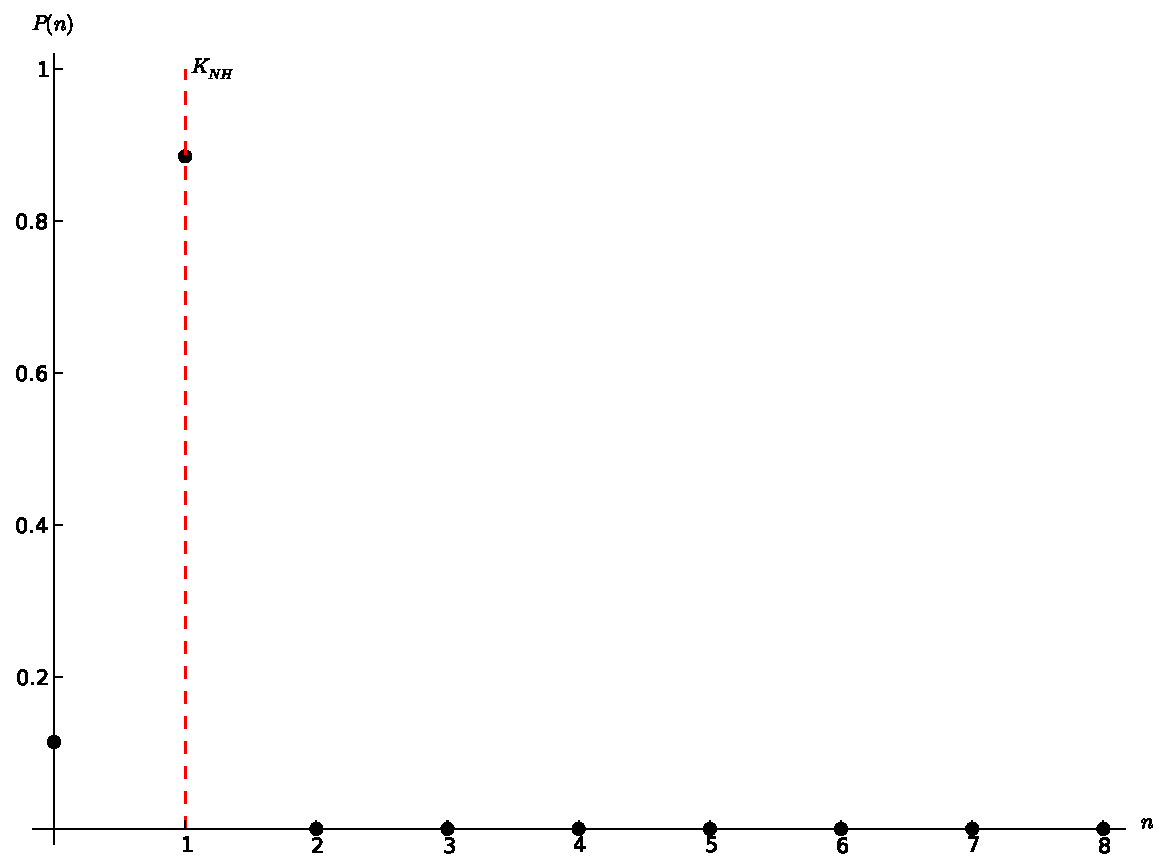
\includegraphics[width=.5\textwidth]{./Images/NH_1_12.pdf}&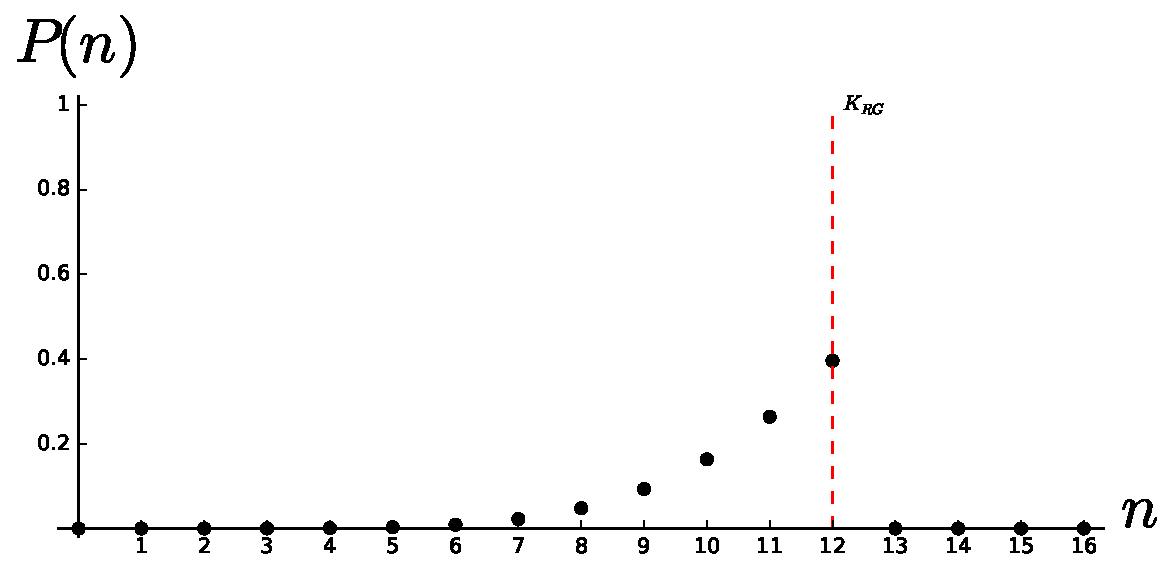
\includegraphics[width=.5\textwidth]{./Images/RG_1_12.pdf}\\
h=\NH&h=\RG
\end{array}
$$
\caption{Steady state probabilities for $h\in\{\NH,\RG\}$ with $(K_{\NH}, K_{\RG})=(1,12)$} \label{steady_state_probs_1_12}
\end{figure}


\subsection{Game Theoretic Model}

Based on the discussion above, the game theoretic model is presented as a synchronous optimisation problem shown in Figure \ref{model1}.

\begin{figure}[!htbp]
\hspace{2cm}For all $h\in\{\text{NH}, \text{RG}\}$ minimise:
$$\left(U_{h}-t\right)^2$$
\hspace{2cm}Subject to:
\begin{align}
0\leq & K_h \leq c_{h}\nonumber\\
&K_h \in  \mathbb{Z}\nonumber
\end{align}
\caption{The optimisation problem underlying the game}\label{model1}
\end{figure}

This game is equivalent to a bi matrix game with restriction to pure strategies where both players aim to get their utilisation as close as possible to a certain target.
As such a Nash Equilibrium is not guaranteed by traditional game theoretical results \cite{Nash1950}, but based on discussions with ABUHB, long term threshold policies are a realistic consideration.

The following result is a sufficient condition for the existence of an equilibrium:\\


\textbf{Theorem.}

Let $f_{h}(k):[1,c_{\bar h}]\to[1,c_h]$ be the best response of player $h\in\{\NH, \RG\}$ to the diversion threshold of $\bar h\ne h$ ($\bar h\in\{\NH, \RG\}$).

If $f_{h}(k)$ is a non-decreasing function in $k$ then the game of Figure \ref{model1} has at least one Nash Equilibrium.


\begin{proof}

The function $f_h$ is well defined as it maximises a continuous function over a finite discrete set (in case of multiple values that minimize $U_h$, it is assumed that $f_h$ returns the lowest such value).

As such if $f_h$ is non-decreasing then it is in fact a stepwise non-decreasing function.
If we consider $f_{\NH}$ and $f_{\RG}$ plotted on the same axis (so that the domain of $f_{\NH}$ is the $x$-axis and the domain of $f_{\RG}$ is the y-axis) it is obvious to see that the functions must intersect at some point as shown in Figure \ref{exampleforproof}.

\begin{figure}[!htbp]
$$\begin{array}{cc}
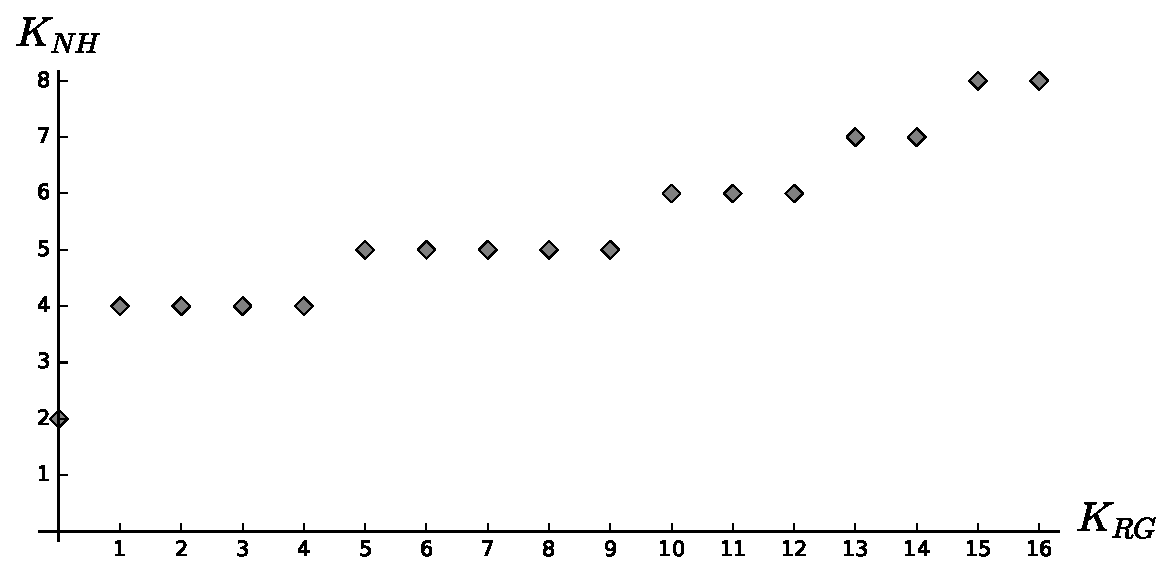
\includegraphics[width=.5\textwidth]{./Images/best_responses_ex_for_proof_NH.pdf}&
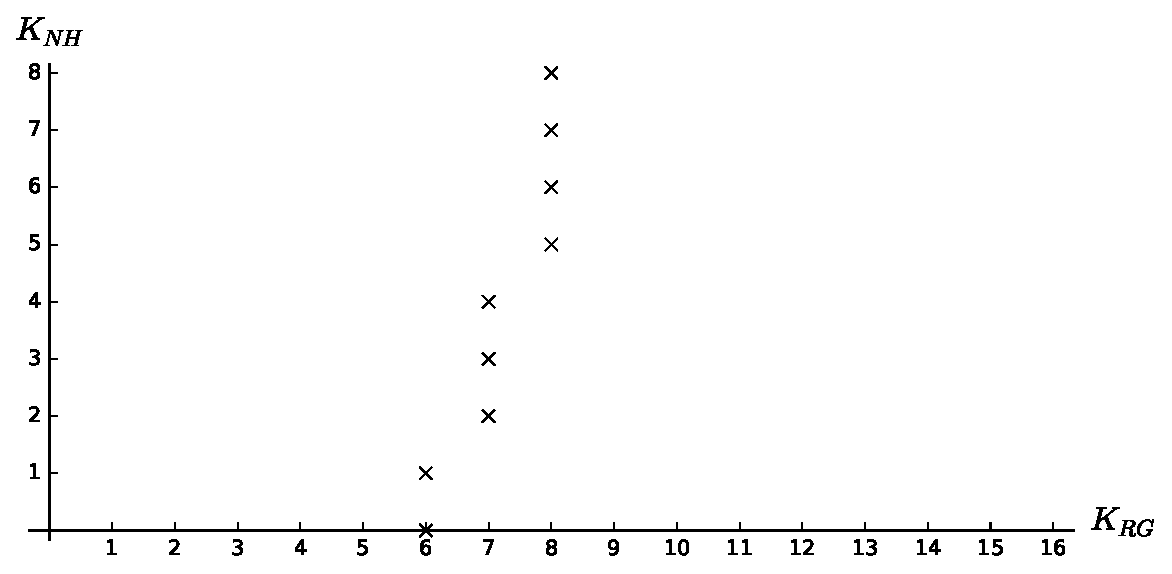
\includegraphics[width=.5\textwidth]{./Images/best_responses_ex_for_proof_RG.pdf}
\end{array}$$
\caption{Plots of $f_{\NH}(K_{\RG})$ and $f_{\RG}(K_{\NH})$}\label{exampleforproof}
\end{figure}

This point of intersection corresponds to a Nash Equilibrium of Figure \ref{model1}.

\end{proof}

This Theorem is in itself not that useful as the properties of $f_{h}$ are difficult to ascertain.
Although the methodology alluded to is how the equilibria are found for the work presented here (exhaustive investigation of best response functions).
The following Lemma will however be of more use in Section \ref{results}.

\textbf{Lemma.}

Using the convention of Figure \ref{arrivalrateregions}:

\begin{itemize}

\item If $\lambda_{\NH}^{(a)}\leq \lambda_{\NH}^{(b)}$ and $\lambda_{\NH}^{(c)}\leq \lambda_{\NH}^{(d)}$ then $f_{\NH}(k)$ is a non-decreasing function in $k$.
\item If $\lambda_{\RG}^{(a)}\leq \lambda_{\RG}^{(c)}$ and $\lambda_{\RG}^{(b)}\leq \lambda_{\RG}^{(d)}$ then $f_{\RG}(k)$ is a non-decreasing function in $k$.

\end{itemize}

Before proving the Lemma the following observation is given:

\textbf{Observation.}

The utilisation $U_h=U_h(\lambda)$ is an increasing function in $\lambda$.

\begin{center}
As the traffic intensity at $h$ increases: $h$ gets busier.
\end{center}


\begin{proof}

A proof for the first part of the Lemma is given (the proof for the second part is analogous).

If $\lambda_{\NH}^{(a)}\leq \lambda_{\NH}^{(b)}$ and $\lambda_{\NH}^{(c)}\leq \lambda_{\NH}^{(d)}$, for given $K_{\NH}$: then as $K_{\RG}$ increases, the arrival rate at NH is non-increasing,
Similarly, for given $K_{{\RG}}$, as $K_{\NH}$ increases the arrival rate at RG is non-decreasing.

Using the above and the previous observation this implies:

\begin{itemize}
    \item The function $U_{\NH}=U_{\NH}(K_{\RG})$ is non-increasing;
    \item The function $U_{\NH}=U_{\NH}(K_{\NH})$ is non-decreasing.
\end{itemize}

A graphical proof of the lemma is then shown in Figure \ref{proof}.

\begin{figure}[!hbtp]
\begin{center}
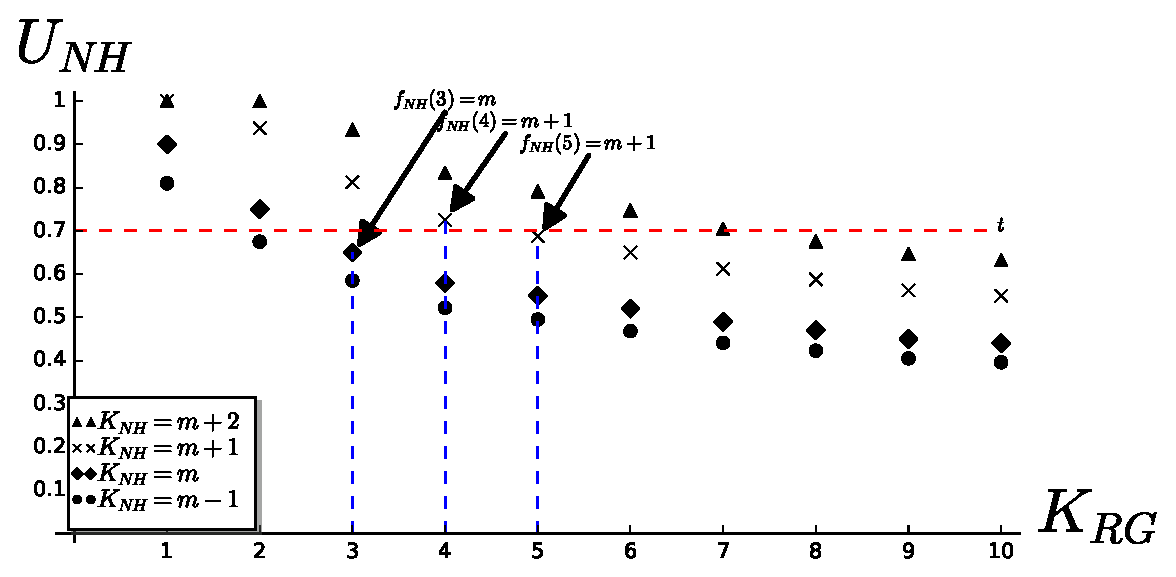
\includegraphics[width=.7\textwidth]{./Images/proof.pdf}
\end{center}
\caption{Graphical proof of the fact that $f_{\NH}(K_{\RG})<f_{\NH}(K_{\RG}+1)$}\label{proof}
\end{figure}

Let $k^*=f_{NH}(K_{\RG})$ for a given $K_{\RG}$.
As $K_{\RG}$ increases, the utilisation $U_{\NH}(k^*)$ will be non-increasing, but it will also be non-increasing for all $k<k^*$.
As $K_{RG}$ increases $\left(U_{NH}(k^*)-t\right)^2$ decreases until $U_{NH}(k^*)=t$ and then increases, however $\left(U_{NH}(k^*+1)-t\right)^2$ will continue to decrease.
Thus, $f_{\NH}(K_{\RG})\geq k^*$ as required.
\end{proof}

The aim of the work presented is to measure the inefficiency created by the removal of central control between CCUs.

We let $\widetilde T$ denote the sum of throughputs at the Nash Equilibrium obtained by solving the game of Figure \ref{model1} (in case of multiple equilibria we take $\widetilde T$ to be the lowest throughput) and let $T^*=\max_{K_{NH}, K_{RG}}\left(T_{NH}+T_{RG}\right)$.

The measure used to quantify inefficiency is the Price of Anarchy (PoA) \cite{Koutsoupias1999,TimRoughgarden}, which is the ratio of the social optimum welfare to the welfare of the worst Nash Equilibrium.
That is, the ratio of the largest social welfare, $T^*$ to the smallest social welfare, $\widetilde{T}$, achieved at any Nash Equilibrium. Thus:

$$\text{PoA}={{T^*}\over{\widetilde{T}}}$$

Note that the classic definition of PoA has been modified here to allow for a maximisation problem.
Social welfare is here considered to be a maximisation of throughput.
An immediate alignment of interests can be obtained by setting $t=1$.
This however would not be in the interest of the hospital (nor necessarily in the interests of patients) as it would imply aiming to run at 100\% utilisation which would not make for a robust system.
\textbf{A sensible value of $t$ is the lowest value of $t$ that ensures a low PoA}.

\section{Results}\label{results}

The game theoretic model of Figure \ref{model1} is solved using exhaustive consideration of best responses whilst taking advantage of the structure identified by the Lemma of Section \ref{queueingandgamemodels}. For any given pair of threshold strategies the matrix equation $\pi Q=0$ is solved by obtaining a basis for the Kernel of $Q$. For the purpose of this paper this is implemented in \cite{sage}.

\subsection{Model 1: Strict diversion}

This model assumes that if the bed occupancy level at both Units exceeds a predetermined threshold, then the admission to the CCU is cancelled (in reality this implies that patients will be admitted to a general ward within the hospital).
Recalling Figure \ref{arrivalrateregions} this implies:

\begin{minipage}[t]{0.5\textwidth}
\small{$$\lambda_{\NH}^{(r)}=\begin{cases}
\lambda_{\NH}, &\text{if }r=a\\
\lambda_{\NH}+\lambda_{\RG},  &\text{if }r=b\\
0, &\text{if }r\in\{c,d\}\\
\end{cases}$$}
\end{minipage}
\begin{minipage}[t]{0.5\textwidth}
\small{$$\lambda_{\RG}^{(r)}=\begin{cases}
\lambda_{\RG}, &\text{if }r=a\\
\lambda_{\NH}+\lambda_{\RG},  &\text{if }r=c\\
0, &\text{if }r\in\{b,d\}\\
\end{cases}$$}
\end{minipage}

We immediately see that the Lemma of Section \ref{queueingandgamemodels} holds and so a Nash Equilibrium for our model exists.

If either CCU chooses their threshold at zero, patients are not admitted at all, and, consequently both Units are closed.

Therefore, the matrix $Q$ has entries $q_{ij}$ as follows:
\begin{equation}
q_{ij}=\begin{cases} u_i\mu_{NH} & \text{ if  } (u_i,v_i)-(u_j,v_j)=(1,0),\\
 v_i\mu_{RG} & \text{ if  } (u_i,v_i)-(u_j,v_j)=(0,1),\\
 \lambda_{\NH} & \text{ if  } (u_i,v_i)-(u_j,v_j)=(-1,0)\text{ and } u_i<K_{\NH} \text{ and } v_i<K_{\RG},\\
 \lambda_{\RG} & \text{ if  } (u_i,v_i)-(u_j,v_j)=(0,-1) \text{ and } u_i<K_{\NH} \text{ and } v_i < K_{\RG},\\
\lambda_{\NH}+\lambda_{\RG} & \text{ if  } \left\{\begin{array}{l} (u_i,v_i)-(u_j,v_j)=(-1,0) \text{ and } u_i<K_{\NH} \text{ and } v_i \geq K_{\RG} \text{ or}\\ (u_i,v_i)-(u_j,v_j)=(0,-1) \text{ and } u_i \geq K_{\NH} \text{ and } v_i < K_{\RG},\\\end{array}\right.\\
0 & \text{ otherwise}.
\end{cases}
\end{equation}

For the parameters of Table \ref{parameter_values_model_1} the best responses are shown in Figure \ref{Fig:best_responses_model1}.
For example, in Figure \ref{Fig:best_responses_model1}a if RG chooses $K_{\RG}=6$, NH has best response $K_{\NH}=8$ .
Similarly, if $K_{\NH}=2$, RG has best response $K_{\RG}=15$.
A Nash Equilibrium for our game is a pair of points that intersect.

\begin{figure}[!htbp]
$$
\begin{array}{cc}
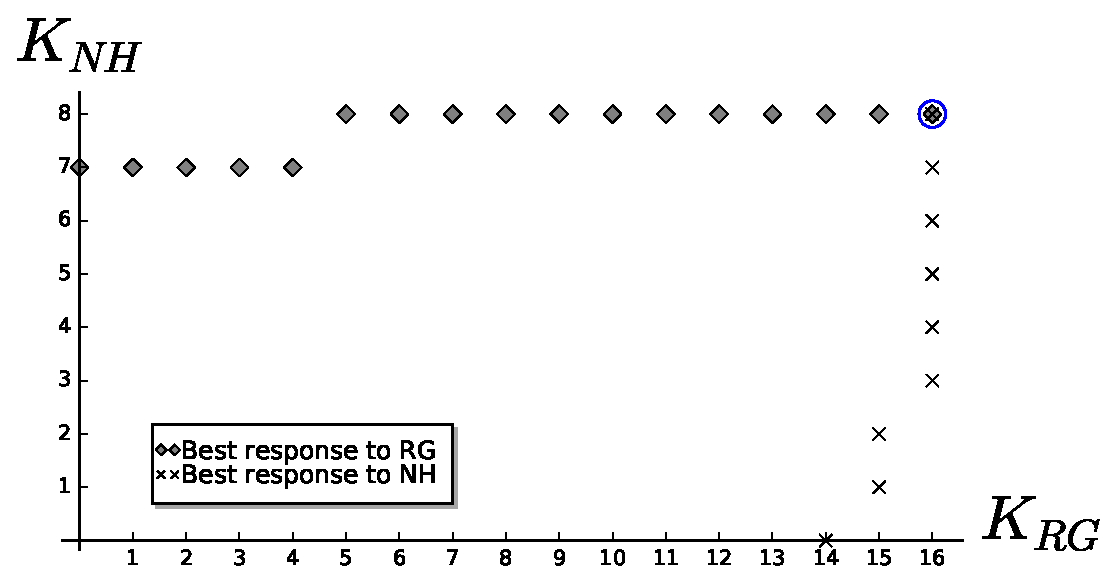
\includegraphics[width=.5\textwidth]{./Images/best_responses_model1.pdf}&
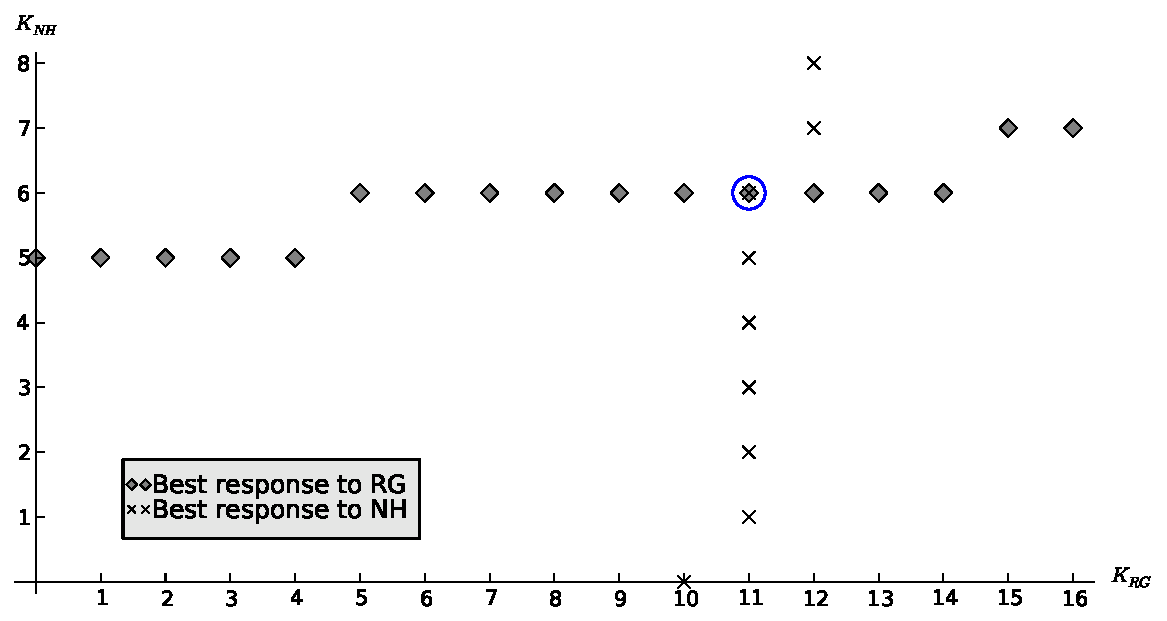
\includegraphics[width=.5\textwidth]{./Images/best_responses_model1_t=0_6.pdf}\\
\text{(a: $t=0.8$)}&\text{(b: $t=0.6$)}
\end{array}
$$
\caption{Best responses for each hospital (a: $t=0.8$; b: $t=0.6$). The point of intersection is circled.} \label{Fig:best_responses_model1}
\end{figure}

For this model the Nash Equilibrium is at $(8,16)$, which gives $\widetilde T=3.65$ and we obtain $T^*=3.65$.
Importantly, a PoA of 1 is not guaranteed for this problem.
For example in Figure \ref{Fig:best_responses_model1}b similar best response behaviour is shown for $t=0.6$ for which the $\text{PoA}=1.18$ (the optimal throughput is again at $(8,16)$).

Whilst removing central control, a certain influence can be exerted by a choice of $t$.
Figure \ref{Fig:target_demand_model1} (note: the non linear scale) and Table \ref{tabletargetdemandm1} show the effect of $t$ and overall demand.
We modify the demand rate from Table \ref{parameter_values_model_1} by taking $\lambda_h \leftarrow \lambda_h(1+x)$ for $-0.9\leq x\leq2$.

\begin{figure}[!htbp]
\begin{center}
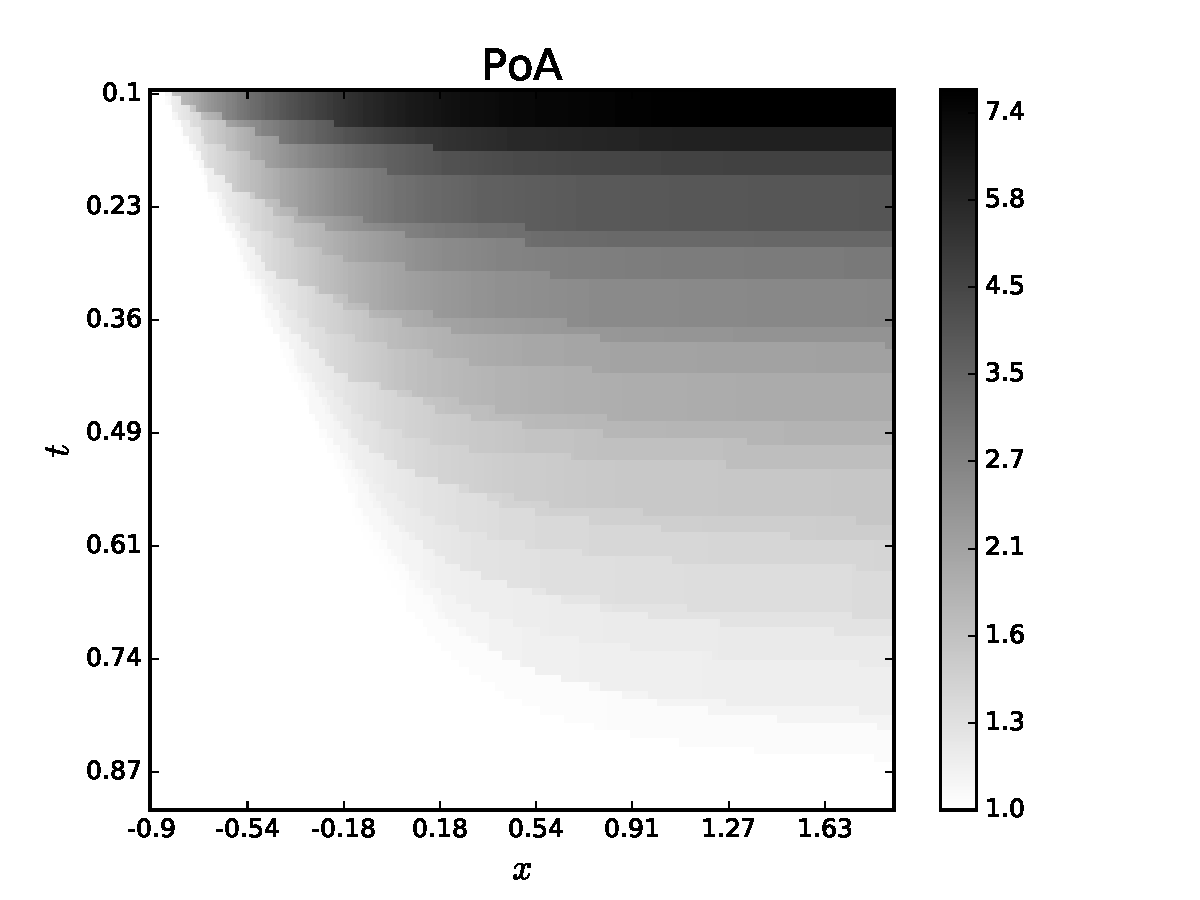
\includegraphics[width=.5\textwidth]{./Images/lnPoAmodel1targetvdemand.pdf}
\end{center}
\caption{PoA for different target and demand rates}\label{Fig:target_demand_model1}
\end{figure}

\begin{table}[!htbp]
\begin{center}
\begin{tabular}{c|ccccccccc}
\toprule
$x$&$t=0.15$&$t=0.27$&$t=0.4$&$t=0.52$&$t=0.64$&$t=0.76$&$t=0.88$&$t=1$\\
\midrule
-0.9&1.0&1.0&1.0&1.0&1.0&1.0&1.0&1.0\\
-0.61&1.64&1.04&1.0&1.0&1.0&1.0&1.0&1.0\\
-0.33&3.27&1.66&1.22&1.0&1.0&1.0&1.0&1.0\\
-0.03&4.43&2.55&1.64&1.34&1.06&1.0&1.0&1.0\\
0.26&5.23&2.99&2.1&1.51&1.28&1.09&1.0&1.0\\
0.55&7.34&3.21&2.25&1.74&1.34&1.16&1.0&1.0\\
0.84&7.6&3.81&2.32&1.79&1.46&1.17&1.03&1.0\\
1.13&7.73&3.88&2.36&1.82&1.48&1.25&1.04&1.0\\
1.41&7.81&3.91&2.61&1.97&1.58&1.26&1.09&1.0\\
1.7&7.86&3.94&2.63&1.98&1.58&1.32&1.14&1.0\\
1.99&7.89&3.95&2.64&1.98&1.59&1.33&1.14&1.0\\
\bottomrule
\end{tabular}
\end{center}
\caption{Numerical values of PoA for different target and demand rates}\label{tabletargetdemandm1}
\end{table}

We see that an extremely large PoA is obtained for $t<0.2$.
For values of $t>0.5$ the PoA is still high: a PoA of 2 corresponds to 100\% less throughput of patients.
These findings seem to give some backing to the targets implemented throughout the NHS \cite{Bevan2006}.

In particular it can be seen that a value of $t>0.8$ becomes imperative for high demand.
The lowest value of $t$ for which gives PoA$=1$ for the actual demand levels ($x=0$) is in fact $t=0.72$.
It is also noted that as demand increases the effect of uncoordinated behaviour increases (and the recommended target also increases) as shown in Figure \ref{mintargetvdemand}.

\begin{figure}[!htbp]
\begin{center}
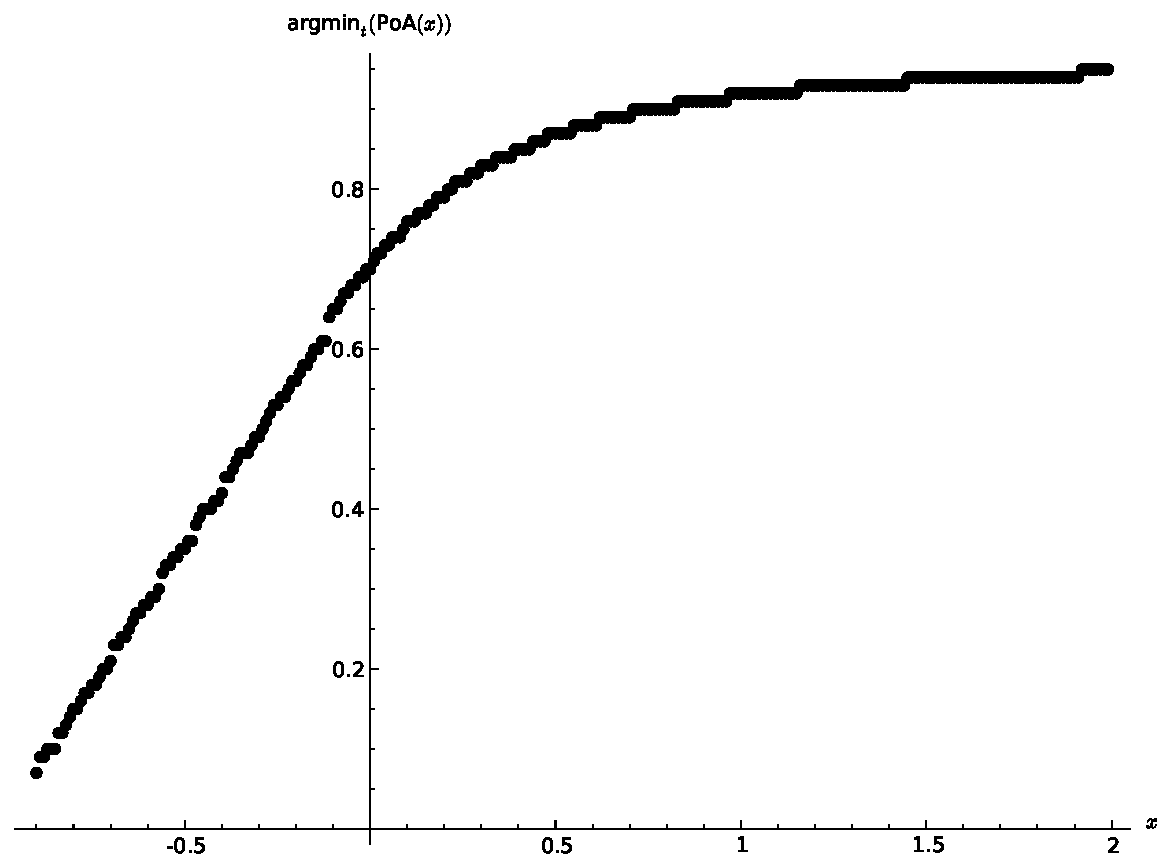
\includegraphics[width=10cm]{./Images/argminPoAmodel1.pdf}
\caption{Lowest value of $t$ ensuring PoA$=1$} \label{mintargetvdemand}
\end{center}
\end{figure}

In this model, there is the potential for both CCUs to divert patients at the same time, and so patients are lost to the entire system. The model of the next section will investigate the effect of not allowing total rejections.

\subsection{Model 2: Soft diversion}

Recalling Figure \ref{arrivalrateregions}, this model assumes:

\begin{minipage}[t]{0.5\textwidth}
\small{$$\lambda_{NH}^{(r)}=\begin{cases}
\lambda_{NH}, &\text{if }r\in\{a,d\}\\
\lambda_{NH}+\lambda_{RG},  &\text{if }r=b\\
0, &\text{if }r=c\\
\end{cases}$$}
\end{minipage}
\begin{minipage}[t]{0.5\textwidth}
\small{$$\lambda_{RG}^{(r)}=\begin{cases}
\lambda_{RG}, &\text{if }r\in\{a,d\}\\
\lambda_{NH}+\lambda_{RG},  &\text{if }r=c\\
0, &\text{if }r=b\\
\end{cases}$$}
\end{minipage}

We immediately see that the Lemma of Section \ref{queueingandgamemodels} holds and so a Nash Equilibrium for our model exists.

This means that if bed occupancy levels at both Units exceed a pre-determined threshold, then diversions do not occur and each CCU has to accommodate their own patients.
In effect we are modelling a certain level of cooperation in this case where CCUs only divert if the other CCU is not busy.

Therefore, the transition matrix $Q$ is obtained from the following transition rates $q_{ij}$:

\begin{equation}
q_{ij}=\begin{cases} u_i\mu_{NH} & \text{ if  } (u_i,v_i)-(u_j,v_j)=(1,0),\\
 v_i\mu_{RG} & \text{ if  } (u_i,v_i)-(u_j,v_j)=(0,1),\\
 \lambda_{NH} & \text{ if  } (u_i,v_i)-(u_j,v_j)=(-1,0) \text{ and }\left\{\begin{array}{l} u_i<K_{NH} \text{ and } v_i<K_{RG}  \text{ or } \\        u_i  \geq K_{NH} \text{ and } v_i  \geq K_{RG},\end{array}\right.\\
 \lambda_{RG} & \text{ if  } (u_i,v_i)-(u_j,v_j)=(0,-1) \text{ and }\left\{\begin{array}{l}u_i< K_{NH}\text{ and }v_i<K_{RG}\text{ or }\\u_i\geq K_{NH}\text{ and }v_i\geq K_{RG}, \\\end{array}\right.\\\\
\lambda_{NH}+\lambda_{RG} & \text{ if  } \left\{\begin{array}{l} (u_i,v_i)-(u_j,v_j)=(-1,0) \text{ and } u_i<K_{NH} \text{ and } v_i \geq K_{RG} \text{ or }\\ (u_i,v_i)-(u_j,v_j)=(0,-1) \text{ and } u_i \geq K_{NH} \text{ and } v_i < K_{RG}, \\\end{array}\right.\\
0 & \text{ otherwise}.
\end{cases}
\end{equation}


As before, Figure \ref{Fig:target_demand_model2} and Table \ref{tabletargetdemandm2} present the PoA for different target values and demand rate changes.

\begin{figure}[!htbp]
\begin{center}
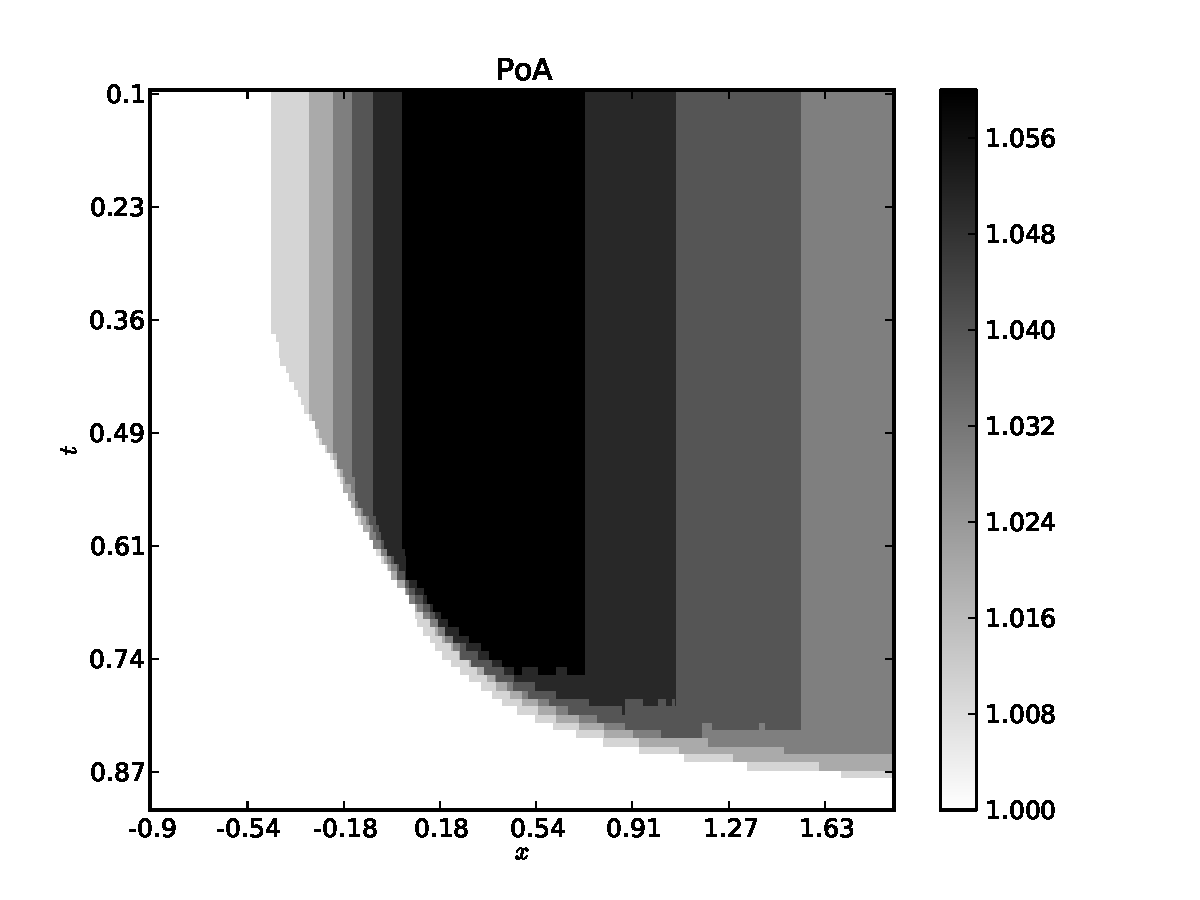
\includegraphics[width=10cm]{./Images/model2targetvdemand.pdf}
\caption{PoA for different target and demand rates for soft diversion} \label{Fig:target_demand_model2}
\end{center}
\end{figure}

\begin{table}[!htbp]
\begin{center}
\begin{tabular}{c|ccccccccc}
\toprule
$x$&$t=0.15$&$t=0.27$&$t=0.4$&$t=0.52$&$t=0.64$&$t=0.76$&$t=0.88$&$t=1$\\
\midrule
-0.9&1.0&1.0&1.0&1.0&1.0&1.0&1.0&1.0\\
-0.61&1.0&1.0&1.0&1.0&1.0&1.0&1.0&1.0\\
-0.32&1.01&1.01&1.01&1.01&1.0&1.0&1.0&1.0\\
-0.03&1.05&1.05&1.05&1.05&1.05&1.05&1.0&1.0\\
0.26&1.06&1.06&1.06&1.06&1.06&1.06&1.06&1.0\\
0.55&1.06&1.06&1.06&1.06&1.06&1.06&1.06&1.01\\
0.84&1.05&1.05&1.05&1.05&1.05&1.05&1.05&1.04\\
1.13&1.05&1.05&1.05&1.05&1.05&1.05&1.05&1.04\\
1.42&1.04&1.04&1.04&1.04&1.04&1.04&1.04&1.04\\
1.71&1.03&1.03&1.03&1.03&1.03&1.03&1.03&1.03\\
1.99&1.03&1.03&1.03&1.03&1.03&1.03&1.03&1.03\\
\bottomrule
\end{tabular}
\end{center}
\caption{Numerical values of PoA for different target and demand rates}\label{tabletargetdemandm2}
\end{table}


We immediately note that the underlying cooperation that is now being forced on our players (divert only if the other player can accommodate the patients) has reduced the PoA.
Note that PoA$=1.02$ still implies a reduced throughput of 2\% which has very large cost implications for a national health service.
A tipping point is now visible as demand increases, this is similar to the profiles shown in \cite{Knight2013} and can be explained as follows:

Also, for very low values of demand, cooperation can be obtained with no target.
\begin{itemize}
    \item When the demand is low, there is no scope for uncoordinated behaviour to be damaging.
    \item When the demand is very high, the system is saturated and once again uncoordinated behaviour has no negative effect in comparison to optimal behaviour.
    \item There is however a region of demand for which there is a high PoA.
\end{itemize}

For example, for $t=0.8$ the PoA starts to rapidly increase for demand changes higher than 0.1, and starts to decrease for a demand change of 0.6; this region will be investigated closely.
Table \ref{table_model2_target_demand} presents results for $t=0.8$ and a demand change from 0.1 to 0.6. For a 50\% increase in demand, without a matching increase in capacity, rational behaviour of CCUs would incur 6\% less patient throughput.

 \begin{table}[!htbp]
\begin{center}
\begin{tabular}{ccccccc}
\toprule
%\textbf{Demand}&\textbf{Nash}&\multirow{2}{*}{\textbf{$\widetilde T$}}&\textbf{Nash NH}&\textbf{Nash RG}&\multirow{2}{*}{\textbf{$T^*$}}&\multirow{2}{*}{\textbf{PoA}}\\
%\textbf{change, $x$}&\textbf{equilibrium}&\textbf{ }&\textbf{throughput}&\textbf{throughput}&\textbf{}&\textbf{}\\
$x$&Nash Equilibrium&$\tilde T$&Nash $T_{NH}$& Nash $T_{RG}$& $T^*$& PoA\\
\midrule
0.1&(8,16)&3.92&1.50&2.42&3.92&1\\
0.2&(8,16)&3.92&1.50&2.42&3.92&1\\
0.3&(6,12)&4.19&1.65&2.54&4.33&1.03\\
0.4&(4,0)&4.22&1.65&2.57&4.48&1.06\\
0.5&(4,0)&4.22&1.65&2.57&4.48&1.06\\
0.6&(0,0)&4.42&1.69&2.72&4.68&1.06\\
\bottomrule
\end{tabular}
\end{center}
\caption{Soft diversion results for $t=0.8$}\label{table_model2_target_demand}
\end{table}


Clearly, as the demand change increases, the Nash Equilibrium thresholds decrease.
This is due to the fact that both CCUs are attempting to divert their patients in less busy states as these states become rarer.
If one CCU diverts early, the other will follow suit (both CCUs incrementally reacting to each other.
As a result the Nash Equilibrium for $x=0.6$ is at $(0,0)$, meaning that each CCU takes care of their own patients.
As the demand increases even further the Nash Equilibrium remains at $(0,0)$ and the PoA decreases.

Figure \ref{mintargetvdemandmodel2} shows the lowest values of $t$ which gives a PoA of 1.
We see that as demand increases this value also increases.
Also, for very low values of demand, cooperation can be obtained with no target.
For the actual demand ($x=0$) a target value of $t=0.72$ is once again recommended.

\begin{figure}[!htbp]
\begin{center}
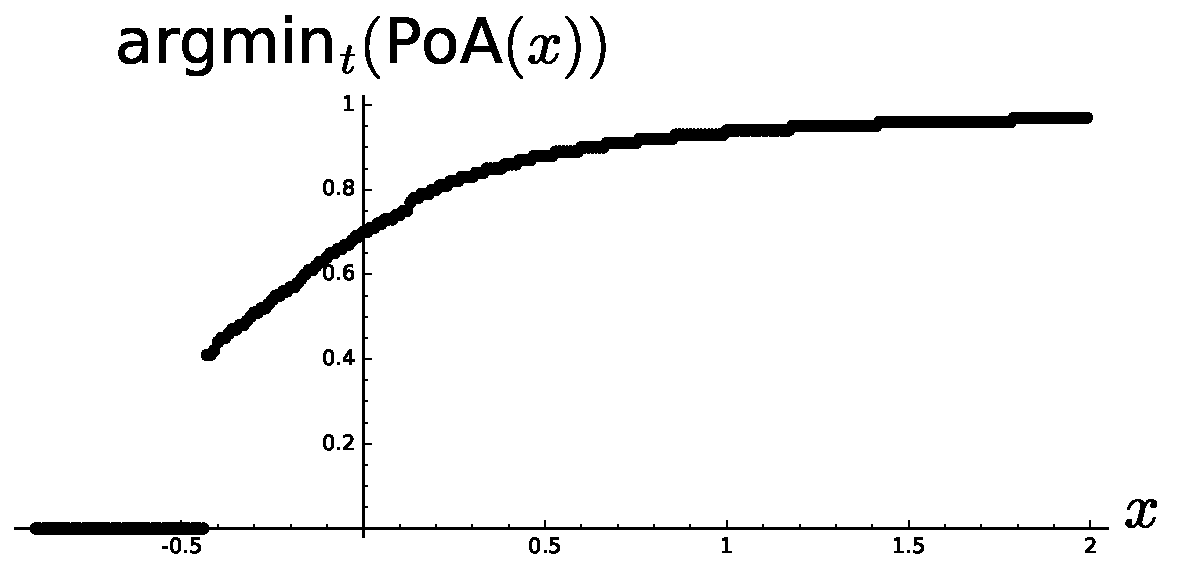
\includegraphics[width=12cm]{./Images/argminPoAmodel2.pdf}
\caption{Lowest value of $t$ ensuring PoA$=1$} \label{mintargetvdemandmodel2}
\end{center}
\end{figure}

\section{Conclusions}\label{conclusions}

In this work a generic game theoretical model has been presented that accounts for the rational actions of two CCUs.
This game theoretic model is underpinned by a queueing model that takes into account the stochastic nature of queueing systems.
This work extends the application of game theoretic models already present in the literature to healthcare \cite{li2002cooperative, xie2006note}.

A result is proved that allows for the assertion of existence of a Nash Equilibrium. This result is then applied to two particular models that are influenced by discussions with a local health board:

\begin{itemize}
\item Strict diversion: patients can be lost to the system if both CCUs declare being in diversion.
\item Soft diversion: if both CCUs are in diversion then they cannot divert their own patients.
\end{itemize}

An analysis of the effect of rational behaviour is given for both of these models in the form of PoA calculations.
The PoA is calculated so as to measure the effect of rational behaviour on overall patient throughput.
High PoAs are found in the case of strict diversion which is to be expected as soft diversion implies a certain level of cooperation.
Importantly a non negligible effect of rational behaviour is calculated for certain policy target values.
A recommendation of setting $t=0.72$ is found across both models. This gives some evidence to a particular target value of maximal utilisation in a two CCU ward setting.

This value of $t$ is investigated against increasing demand and is shown to be increasing in overall demand across the system.
Investigating demand is akin to investigating the capacity of the CCUs and as shown in Figure \ref{capacity}: if capacity is not sufficient rational behaviour can have a very damaging effect on overall patient throughput.

\begin{figure}[!htbp]
$$\begin{array}{cc}
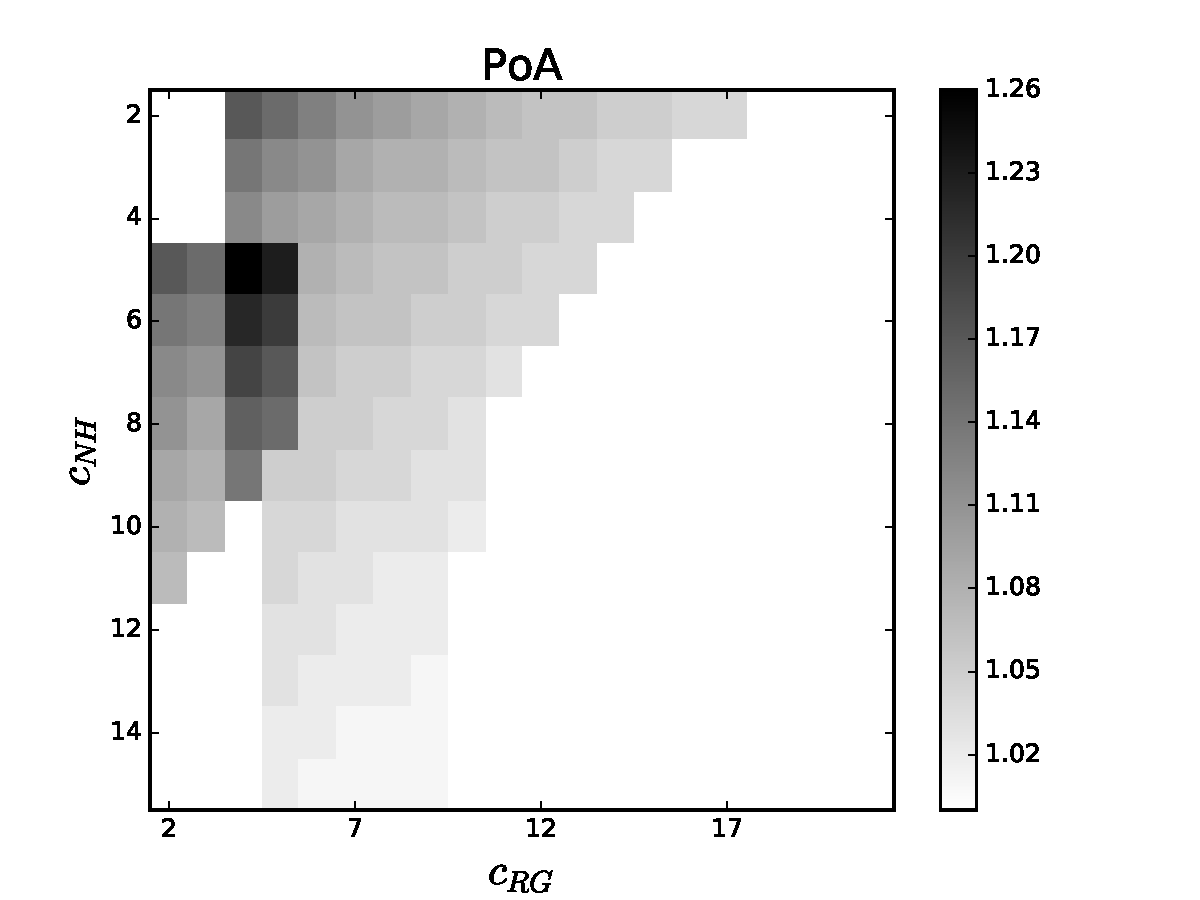
\includegraphics[width=.5\textwidth]{./Images/model1capacity.pdf}&
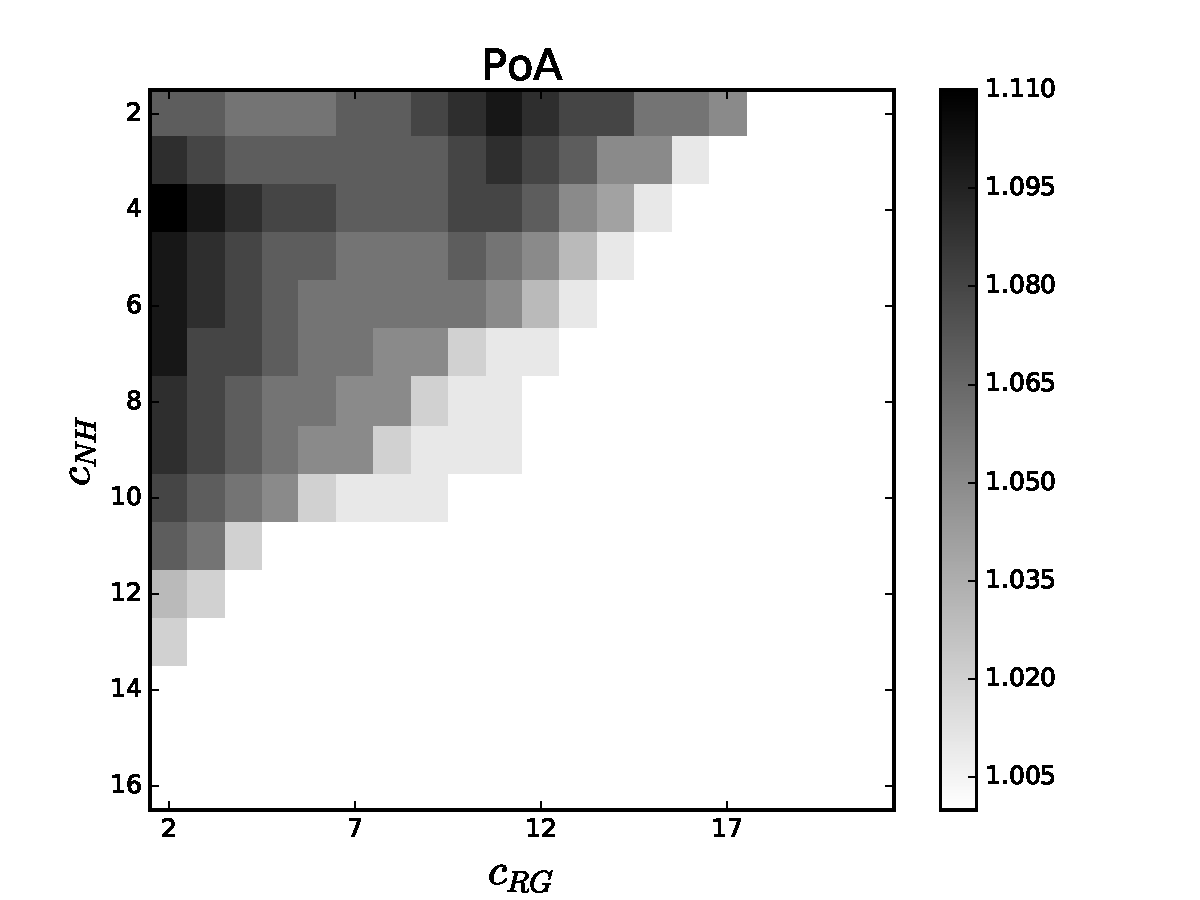
\includegraphics[width=.5\textwidth]{./Images/model2capacity.pdf}
\\
\text{a: Strict diversion}&\text{b: Soft diversion}\\
\end{array}$$
\caption{The effect of capacity on the PoA}\label{capacity}
\end{figure}

It is vital to acknowledge the limitations of the work presented:

\begin{itemize}
    \item The assumptions as to the strategy space of our players is restrictive: a single threshold policy might not be optimal (although it is present in various pieces of literature on optimal control of queueing systems: \cite{naor1969regulation, shone2013comparisons});
    \item This model only assumes the presence of two players however in reality the system has a variety of stakeholders. Multi player systems could be worth considering;
    \item The restriction to pure strategies is influenced by discussions with ABUHB and also does not detract from the results presented thanks to the Theorem and Lemma of Section \ref{queueingandgamemodels}.  However, allowing for mixed strategies could also be of interest.
\end{itemize}

Despite these limitations the work presented here gives a strong analytical evidence as to the use of policies in a decentralised healthcare environment.
Further work could involve the investigation of patient survival instead of throughput as utility.
This would be similar to work such as \cite{erkut2008ambulance, knight2012ambulance}.

The code used in this work can be found here: \url{https://github.com/drvinceknight/Measuring_the_price_of_anarchy_in_ccu_interactions}.
The graphics for this paper were obtained using \cite{Hunter:2007, sage} a worksheet with the data and code used for the plots can be found here: \url{https://sage.maths.cf.ac.uk/home/pub/122/}.

\newpage
\bibliographystyle{plain}
\bibliography{library}

\end{document}
